%!TEX root = ../thesis.tex
%*******************************************************************************
%*********************************** Third Chapter *****************************
%*******************************************************************************

\chapter{Bioelectrical impedance plethysmography}  %Title of the First Chapter
\label{chapter impedance}

\ifpdf
    \graphicspath{{Chapter3/Figs/Raster/}{Chapter3/Figs/PDF/}{Chapter3/Figs/}}
\else
    \graphicspath{{Chapter3/Figs/Vector/}{Chapter3/Figs/}}
\fi

One of the purposes of this work is to produce a device capable of detecting, measuring, and quantifying changes in the venous and arterial circulation continuously. The most common method to measure these changes is known as plethysmography. With this information, it is possible to quantify changes in blood volume which can also be translated into blood flow rate.  But before going deep into the design of this device, it is necessary the principles of operation and theories behind this technology. 

This chapter describes the principles behind bioelectrical impedance plethysmography in more detail. But before getting to that point, the effect of alternate current (AC) will be described to identify the safe limits when applied to the human body. Then, the basics of the electrical impedance in conductors are described including how electrical current distributes in volumes. Later, the electrode-skin interface is explored to comprehend how electric current conduction converts into ionic conduction. 

The bioelectrical impedance section explores more in detail the effect of AC in the human body when interacting with cells and how data is interpreted. A scope of the latest bioelectrical impedance technology will be described including its essential components and methods to measure it. With this basic concept understood, bioelectrical impedance plethysmography will be illustrated showing the principles behind it and the examining the signals that this kind of instrument can produce.  

%********************************** % Sixth Section  *************************************
\section{Electrical current in the human body} %Section - 3.7
\label{section impedance current in body}
Injecting electric current in biological tissue requires some safety measurements so as to guarantee the patients welfare. Driving current into the human body may cause unpleasant effects like heating, electrolysis at the electrode–tissue interface or neuromuscular stimulation \cite{bertemes2002tissue, martinsen2011bioimpedance}. The latter being the most dangerous because it controls blood circulation and respiration. Levels of current sensation changes from person–to–person, sex and also depend on the electrode’s geometry. However, Brown et al. \cite{brown1998medical} have established a threshold current where sensation increases when frequency rises as shown in Figure \ref{fig:threshold sensation}. It has been recognised the frequency dependency of the human body. The maximum sensitivity of the nervous system is in the frequency range between \SIrange[scientific-notation = engineering]{10}{1000}{\hertz}. At frequencies above \SI{1}{\kilo\hertz} sensitivity is considerably reduced and above \SI{100}{\kilo\hertz} it is entirely imperceptible. In fact, the heat effect is so high at these frequencies that electro-surgical devices use it. Square waves are not recommended because they have the DC and AC effect in one signal where the duration of the pulse an important parameter to be controlled \cite{martinsen2011bioimpedance}.

\begin{figure}[!htpb]
	\centering
	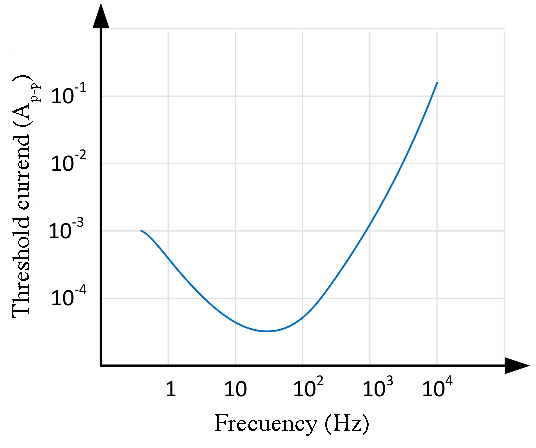
\includegraphics[width=0.45\textwidth,keepaspectratio]{figure14}    
	\caption[Threshold current sensation vs. frequency]{Threshold current sensation vs. frequency. Adapted from \cite{brown1998medical}}
	\label{fig:threshold sensation}
\end{figure}

The table \ref{table:current in body} shows different levels of electric current tolerance of the human body. These effects are mostly dependant on current rather than frequency. When frequencies are above \SI{100}{\kilo\hertz} especially on the radio–frequency (RF) range (\SIrange[scientific-notation = engineering]{400000}{3000000}{\hertz}) the heating effect of the tissue is more common. As can be seen, to avoid patient’s discomfort, currents bellow \SI{5}{\milli\ampere} must be used in BIA device.

\begin{table}[!htpb]
	\caption{Effect of electric current in the human body}
	\centering
	\label{table:current in body}
	\begin{tabular}{lp{0.525\textwidth}}
		\toprule
		\textbf{Current Level}                &         \textbf{Effect}          \\ \midrule
		
		< \SI{1}{\milli\ampere}                &  
		\begin{tabular}[t]{@{\textbullet~}p{0.5\textwidth}@{}} 
			Usually not perceptible 
		\end{tabular}
		\\\midrule
		\SI{1}{\milli\ampere}                  &  
		\begin{tabular}[t]{@{\textbullet~}p{0.5\textwidth}@{}} 
			Threshold of current perception \\
			Tingling sensation
		\end{tabular}
		\\\midrule
		\SI{5}{\milli\ampere}                  &  
		\begin{tabular}[t]{@{\textbullet~}p{0.5\textwidth}@{}} 
			Sensory nerve stimulation\\ 
			Shock sensation 
		\end{tabular}
		\\\midrule
		\SIrange{6}{25}{\milli\ampere} (Women) &  
		\begin{tabular}[t]{@{\textbullet~}p{0.5\textwidth}@{}} 
			Painful electric shock \\ 
			Lack of muscular control 
		\end{tabular}
		\\\midrule
		\SIrange{9}{30}{\milli\ampere} (Men)   &  
		\begin{tabular}[t]{@{\textbullet~}p{0.5\textwidth}@{}} 
			Difficult to let go – freezing current range \\
			High muscle contraction
		\end{tabular}	
		\\\midrule
		\SIrange{50}{150}{\milli\ampere}       &  
		\begin{tabular}[t]{@{\textbullet~}p{0.5\textwidth}@{}} 
			Extreme pain \\
			Possible respiratory arrest \\
			Possible ventricular fibrillation (VF) \\
			Sever muscular contraction \\
			Possibly death
		\end{tabular}
		\\\midrule
		\SIrange{1}{4.3}{\ampere}              &  
		\begin{tabular}[t]{@{\textbullet~}p{0.5\textwidth}@{}} 
			Heart’s electric coordination compromised \\
			Muscular contraction and nerve damage \\
			Death likely 
		\end{tabular}
		\\\midrule
		\SI{10}{\ampere}                       & 
		\begin{tabular}[t]{@{\textbullet~}p{0.5\textwidth}@{}} 
			Cardiac arrest \\
			Severe burns \\
			Highly probability of death
		\end{tabular}
		\\\bottomrule                            
	\end{tabular} 
\end{table}

Recommendations, guidelines and norms for patient safety are contained in international standards compiled by the International Electrotechnical Commission (IEC). The standard applicable to medical equipment or equipment to be used with humans is referenced as IEC 60601 or IEC 601 for short. Some of the recommendations regarding safety are expressed as follows: first, the commission considers any frequency below \SI{0.1}{\hertz} as direct current, in order to avoid ulcers created by electrode–skin interface this type of current should be limited to \SI{10}{\uArms}. Moreover, for frequencies up to \SI{1}{\kilo\hertz}, it is recommended to limit current at \SI{100}{\uArms}. Secondly, avoiding nerve stimulation is crucial for patient safety; at frequencies above \SI{1}{\kilo\hertz}, muscular stimulation is very difficult. Therefore is recommended use frequencies above this value. Thirdly, one important recommendation of the standard is that the maximum current flowing through skin contact must be limited to \SI{0.5}{\milli\ampere} with single fault equipment \rvmynote{I have to check this, becuase it rises questions}. Lastly, as explained before in the RF range tissue could be heated, tissue burn can be avoided by limiting the current density and duration, for instance, is recommended using densities of less than \SI{1}{\milli\ampere\per\milli\meter\squared}. In practical applications of current vs. frequency, for frequencies above \SI{1}{\kilo\hertz}, the Commission has established the equation \ref{eq:current body} to calculate the maximum root–mean–square current when this is less than \SI{10}{\mArms}.

\begin{align}
	\label{eq:current body}
	I_{MAX(RMS)} = 10^{-7}.f
\end{align}

where $f$ is the frequency of the measurement.

\section{Electrical impedance principle}
\label{section impedance principle}
%https://books.google.co.uk/books?id=M74ecVj5q9UC&printsec=frontcover&dq=inauthor:%22Luca+Callegaro%22&hl=en&sa=X&ved=0ahUKEwjMyPSt5MnSAhUJJcAKHZAPBGcQ6AEIHDAA#v=onepage&q&f=false
From the electrical point of view, impedance is defined as the opposition that a medium presents to either an alternating current (AC) or voltage (see figure \ref{fig:impedance}) \cite{callegaro2012electrical}. Impedance is equal to the complex ratio between electrical voltage and current. The result from this mathematical fraction is a complex number which is known as symbol $Z$ (see equation \ref{eq:Z magnitude}). This comprises of a resistance (also known as conductance) and/or reactance value, commonly represented by the letters $R$ and $X$ respectively. Hence, the impedance measurement can be expressed as a relation of the output magnitude and the phase difference between the real and imaginary part as shown in equation \ref{eq:phasor} and it can be plotted in the complex plane as shown in figure \ref{fig:complex impedance}.

\begin{figure*}[!htpb]
	\centering
	\begin{subfigure}[t]{0.4\textwidth}
		\centering
		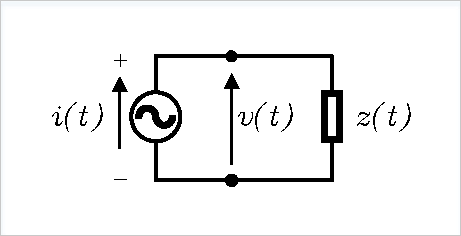
\includegraphics[width=6cm,trim={0.05cm 0.05cm 0.05cm 0.15cm},clip,keepaspectratio]{figure0a}    
		\caption{Current driven impedance}
		\label{fig:impedance a}
	\end{subfigure}
	~
	\begin{subfigure}[t]{0.4\textwidth}
		\centering
		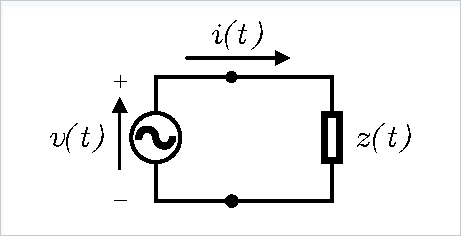
\includegraphics[width=6cm,trim={0.05cm 0.05cm 0.05cm 0.15cm},clip,keepaspectratio]{figure0b}    
		\caption{Voltage driven impedance}
		\label{fig:impedance b}
	\end{subfigure}
	\caption[Impedance representation from two-terminal element]{Schematic of the electrical impedance. The three elements requires are the voltage $v(t)$, the alternating current $i(t)$ and the opposition to the current ($z(t)$). The impedance can be driven by either current or voltage.}
	\label{fig:impedance}
\end{figure*}

\begin{align}
	\label{eq:phasor}
	Z = \lvert Z \rvert  \angle \phi
\end{align}

There are different ways to represent impedance. However, bioelectrical impedance can be described by either resistance ($R$) or reactance ($X$). Where the resistive part represents the real part of the measurement and the reactance the imaginary one. Therefore, the impedance magnitude can be written as a function in these two values as shown in equation \ref{eq:Z magnitude}.

\begin{figure}[!htpb]
	\centering
	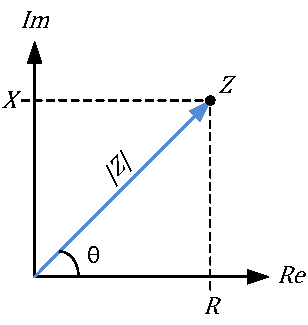
\includegraphics{figure_2}    
	\caption[Complex representation of impedance]{Plot of the impedance in the complex plane.}
	\label{fig:complex impedance}
\end{figure}

\begin{gather}
	\label{eq:Z magnitude}
	Z = Z' + Z'' = R + jX = \lvert Z \rvert e^{j\theta}\\
	|Z| = \sqrt{Z Z^{*}} = \sqrt{R^2 + X^2} \\
	\theta = tan^{-1}\frac{X}{R} \\
	\label{eq:resistance}
	R = \lvert Z \rvert cos(\theta) \\
	\label{eq:reactance}
	X = \lvert Z \rvert sin(\theta)
\end{gather}

As can be seen, when the angle difference of the impedance is \SI{0}{\degree}, the load is completely resistive. In contrast, when the phase difference is \SI{90}{\degree} the load is purely reactive. From the previous equations it is possible to represent impedance in the complex plane as shown in figure \ref{fig:complex impedance}.

Another way to express and analyse impedance is with sinusoidals. For instance, when a sinusoidal steady-state waveform injects a current $i(t) = I_A cos(\omega t)$ to an unknown load, the response is a shifted sinusoidal waveform with a potential equivalent to $v(t) = V_B cos(\omega t + \phi)$. Figure \ref{fig:impedance wave} shows the representation of both waveforms. Hence, the impedance can be expressed as the ration of these two quantities based on Ohm's law (see equation \ref{eq:ohm}).

\begin{align}
	\label{eq:ohm}
	Z = \frac{V}{I}
\end{align}

\begin{figure}[!htpb]
	\centering
	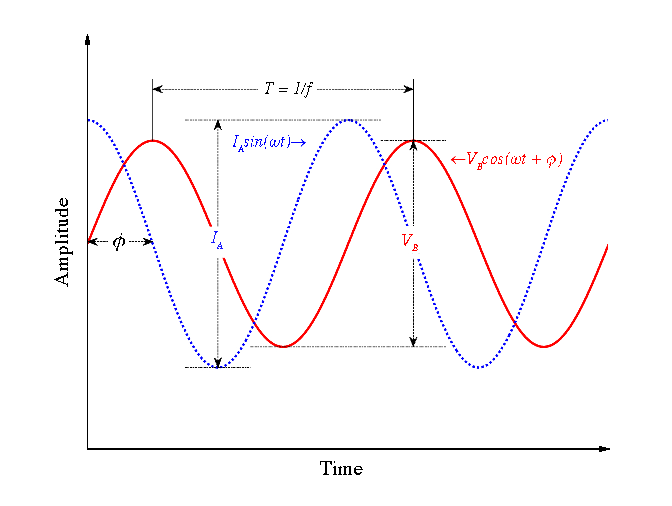
\includegraphics[width=0.8\textwidth,keepaspectratio, trim={0cm 0cm 0cm 0cm},clip]{figure_1}    
	\caption[Impedance waveforms]{Waveform plot of a current ($I_A cos (\omega t)$) compared to the potential representation ($V_B cos (\omega t + \phi)$) of an unknown load.}
	\label{fig:impedance wave}
\end{figure}


However, performing mathematical operations with trigonometry identities could be quite tedious. Therefore, equivalent methods are used to analyse impedance in an electric circuit. Using Euler's formula is possible to express trigonometric functions in order of $e$. The equation \ref{eq:euler} shows the relation between both entities.

\begin{equation}
	\label{eq:euler}
	e^{j\omega t} = cos(\omega t) + j sin(\omega t)
\end{equation}  

Therefore, voltage and current can be rewritten in the form of complex exponential thanks to Euler's equation. 

\begin{align}
	\label{eq:volatge euler}
	v(t) = V_B cos(\omega t + \phi) = V_B(e^{j(\omega t + \phi)}) \\
	\label{eq:current euler}
	i(t) = I_A cos(\omega t) = I_A(e^{j\omega t})	
\end{align}

Using Ohm equation \ref{eq:ohm} is possible to calculate the resultant impedance of the waveforms. Therefore, the expression using complex exponentials would be equal to:

\begin{align}
	\label{eq:complex Z}
	Z = \frac{v(t)}{i(t)} = \frac{V_B(e^{j(\omega t + \phi)})}{I_A(e^{j\omega t})} = \frac{V_B}{I_A} e^{j\phi}
\end{align}

Then, by the Euler's equation is possible deduct the real and imaginary parts of the complex exponential of equation \ref{eq:complex Z}.

\begin{align}
	\label{eq:complex Z2}
	Z = \frac{V_B}{I_A} e^{j\phi} = \frac{V_B}{I_A}(cos(\phi) + j sin(\phi)
\end{align}

By the principle of superposition is possible to assume that the real an imaginary components of impedance are given by the following formulas, which are equivalents to the ones obtained with phasor analysis equations	\ref{eq:resistance} and \ref{eq:reactance}.

\begin{align}
	\label{eq:R Z}
	Z' = R = \frac{v(t)}{i(t)} = \frac{V_B}{I_A}cos(\phi) \\
	\label{eq:X Z}
	Z'' = X = \frac{v(t)}{i(t)} = \frac{V_B}{I_A}sin(\phi)
\end{align}

As a conclusion, it is possible to obtain real and imaginaries values of impedance if the maximum amplitude of the voltage ($V_B$) and current ($I_A$) are known, as well as their difference in phase ($\phi$). 

%********************************** % Fourth Section  *************************************
\section{Current distribution in conductors (Geselowitz theorem)}  %Section - 3.4
\label{section impedance Geselowitz}
Geselowitz \cite{geselowitz1971application} studied the change in conductivity within a constant geometry. In short, his analysis applied the lead field theory into electrical impedance. Simplifying the origin of the equation, the total impedance of the whole volume is equivalent to the sum of all the small impedances within each small volume $dV$ \cite{martinsen2011bioimpedance}.

\begin{figure}[!htpb]
	\centering
	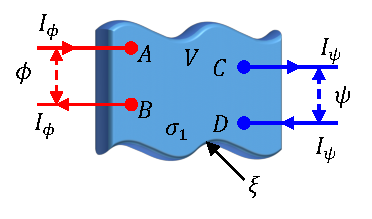
\includegraphics[width=6.3cm,keepaspectratio]{figure9}    
	\caption[Volume conductor with 4 electrodes]{Volume conductor $V$ of conductivity $\sigma_1$. A:B represent current injection electrodes and C:D are sensing electrodes.}
	\label{fig:volume}
\end{figure}

The analysis of this equation starts from the study of the four-electrode measurement and the change in conductivity of the internal region of a volume conductor \cite{bertemes2002tissue}. From Figure \ref{fig:volume} is assumed that a volume conductor is electrically linear and surrounded by an insulator $\xi$. If the internal conductivity changes from $\sigma_1$ to $\sigma_2$ (equivalent to $\sigma_1+\Delta \sigma$) then the potential field of the current injection will change from $\phi$ to $\phi \prime$ (equal to $\phi+\Delta \phi$) but sensing potential field $\psi$ will remain unchanged. Then the field equation can be written as follows:

\begin{align}
	\label{eq:potential field}
	\int_{\Omega} \sigma . (\phi - \phi \prime) . \nabla \psi d \overline{S} = \int_{V} (\sigma_1 - \sigma_2).(\nabla \phi \prime \bullet \nabla \psi).dV 
\end{align}

By replacing the terms by the equivalents, the equation can be rewritten according to the next equation.

\begin{align}
	\label{eq:potential field2}
	- \Delta \phi_{CD} . (-I_{\psi}) = - \int_{V} \Delta \sigma . [\nabla (\phi + \Delta \phi) \bullet \nabla \psi].dV
\end{align}

The impedance change can be deducted by dividing the function by the currents involved $I_{phi}$ and $I_{\psi}$. As a result, the Geselowitz’s equation is equivalent to:

\begin{align}
	\label{eq:Geselowitz}
	\Delta Z = \frac{\Delta \phi_{CD}}{I_\phi} = - \int_V \Delta \sigma (x,y,z).\bigg[\frac{\nabla(\phi + \Delta \phi)}{I_{\phi}} \bullet \frac{\nabla \psi}{I_{\psi}}\bigg].dV
\end{align}

The previous equation is the key to calculating the change in impedance in a volume within defined boundaries. However, this only applies to homogeneous and isotropic volume conductors. This equation can be simplified if is assumed that a unit of current passes through and the volume conductor can be denoted by a number of discrete elements of uniform conductivity in three dimensional space ($x,y,z$). As a result, the equitation can be simplified as follows:

\begin{align}
	\label{eq:Geselowitz2}
	\Delta Z = - \Delta \sigma \cdot \int_V \nabla(\phi + \Delta \phi) \bullet \nabla \psi . dV = - \Delta \sigma \cdot S
\end{align}

where $S$ represents the sensitivity matrix in three dimensions, and it is independent of conductance. Calculate this variable requires a series of assumptions such as the initial conductivity distribution is uniform \cite{dehghani1999incorporating}. This document is not centred in the mathematical analysis of the sensitivity S but to deduct that impedance changes are directly related to the change of geometry of the segment. Several studies have been proof that sensitivity varies according to the electrodes position and geometry as researched by Filho \cite{bertemes2002tissue}.

%********************************** % Second Section  *************************************
\section{Electrode-skin interface}  %Section - 3.3
\label{section impedance electrodes}
Electrodes play a key feature in a bioelectrical impedance system. The right electrode geometry, distance and material may influence in the readings from a biological sample. Consequently, it is needed to use electrodes that have minor impedance compared to the one from the subject under test. Currently, most common materials used in bioelectrical impedance are platinum (\textit{Pt}), gold (\textit{Au}) or stainless steel. Other independent variables such temperature, ionic tissue contents and protein adhesion influence in the change of electrode impedance~\cite{ivorra2003bioimpedance,martinsen2011bioimpedance}. The geometry of the electrode also affects its resistance ($R$) as explain by ohm’s law in equation \ref{eq:resist}.

\begin{align}
	\label{eq:resist}
	R = \rho \frac{L}{A}
\end{align}

where $\rho$ is the electrical resistivity of the material, $A$ is the area of the electrode and $L$ its longitude or thickness. As it can be noticed, the resistance ($R$) reduces when the area ($A$) of the electrode increases. However, the total resistance ($R$) is directly proportional to the electrodes length. 

When an electrode adheres to the skin, and electrical current passes through, a physical effect takes place. First, there is an electrical charge change from electronic to ionic conduction because inside the body the latter is only possible. Second, at the electrode–tissue boundary an electrochemical reaction follows, called electrolysis. This effect creates a “double layer capacitance (DLC)” (see figure \ref{fig:DLC}) that as its name indicates, adds a capacitive effect to boundary \cite{lvovich2012impedance}. Consequently, applying an AC waveform inverts the electrode’s polarity during each cycle minimising this capacitive effect. However, this is a frequency dependent development, which means that at low frequencies can be quite notorious \cite{bertemes2002tissue}.  

\begin{figure}[!htpb]
	\centering
	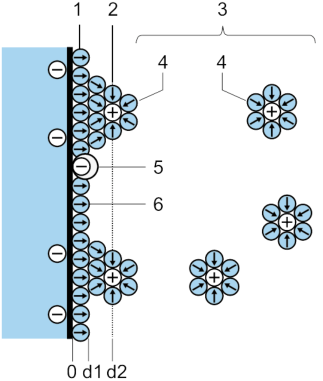
\includegraphics[width=5.5cm,keepaspectratio]{figure7}    
	\caption[Dual layer representation on an electrode]{Schematic representation of a double layer on an electrode (BMD) model. 1. Inner Helmholtz plane, (IHP), 2. Outer Helmholtz plane (OHP), 3. Diffuse layer, 4. Solvated ions (cations) 5. Specifically adsorbed ions (redox ion, which contributes to the phase shift element). Image from \cite{lvovich2012impedance}}
	\label{fig:DLC}
\end{figure}

An electric circuit model can represent the electric–tissue interface; this simplified electric representation is shown in figure \ref{fig:e-t circuit}. In more detail, this model is characterised by a charge transfer resistance ($R_{CT}$) in parallel with interface’s impedance ($Z_{CPE}$) in series with the tissue impedance ($Z_t$).  Some authors have defined the interface’s impedance as either a constant phase angle impedance ($Z_{CPA}$) \cite{franks2005impedance} or constant phase element ($C_{PE}$) \cite{barsoukov2005impedance,mcadams2006characterization}. 

\begin{figure}[!htpb]
	\centering
	\begin{circuitikz}
		\draw[american](0,0) 
		to[short, n=met] (2,0)
		to[short, o-*] (2,0) -- (2,1)
		to[generic=$Z_{CPE}$] (4,1) -- (4,0)
		to[short, o-*] (4,0)
		to[generic=$Z_t$, n=res] (6,0)
		(2,0) -- (2,-1)
		to[R=$R_{CT}$](4,-1)--(4,0)
		
		(met.s) node[below]{Metal}
		(res.s) node[below]{Tissue}
		;
	\end{circuitikz}   
	\caption[Equivalent circuit electrode–tissue interface]{Equivalent circuit electrode–tissue interface (Adapted from Franks~\cite{franks2005impedance})}
	\label{fig:e-t circuit}
\end{figure}

The value of $Z_{ZPA}$ can be calculated from the following empirical equation \ref{eq:zcpa} given by McAdams~\cite{mcadams1995linear}.

\begin{align}
	\label{eq:zcpa}
	Z_{CPA} = K(j\omega)^{-\beta}
\end{align}

where $K$ is a measure of the magnitude of $Z_{CPA}$, $\beta$ is a constant ($0 \leq \beta \leq 1$) representing inhomogeneities in the surface (typically \num{0.8} for many biomedical electrode systems) and $\omega = 2\pi f$. When $\beta = 1$, $Z_{CPE}$ is equivalent a purely capacitive impedance element \cite{franks2005impedance,mcadams2006characterization,mcadams1995linear}.

Electrodes are also a source of error when taking measurements. Some blunders can even distort the original signal; such as thermal noise also known as Johnson-Nyquist noise. This type of noise is entirely inherent to the electrode and also depends on other external variables.  The equation \ref{eq:nyquist noise} represents the level of noise coming from the electrode~\cite{mcadams1995linear}.

\begin{align}
	\label{eq:nyquist noise}
	V_n(rms)=\sqrt{(4 K_b T R \Delta f)}
\end{align}

where $K_b$ is Boltzman constant, $T$ is absolute temperature, $R$ is the electrode’s resistance and $\Delta f$ is the bandwidth of the measurements. 

In summary, it can be appreciated that the noise ($V_n(rms)$) is directly proportional the bandwidth’s measurements ($\Delta f$). At high operating frequency is expected a higher the level of noise. In the case of impedance plethysmography the bandwidth is in the lower range of \si{\kilo\hertz} which minimises the effect of the Johnson-Nyquist noise.

Another source of errors caused by electrode can be derived from their position in the body, lack of surface contact or mismatch in materials and geometries. Therefore, to improve and maximise the area of contact, some electrodes requires of conductive gel. It has been demonstrated that using commercially available electrodes for electrocardiogram (ECG) purposes does provide good impedimetric readings, compared to specially designed electrodes~\cite{caicedo2012use}.

An experiment using this type of electrodes was carried out to determine whether removing one or four electrodes and then put them back in the same position could produce errors in readings. It was found that putting electrodes away and then adhere them again within an extended period represented a minimum change in impedance readings. Most of the changes were presented in variations in the geometry of the segment under test caused by the electrode's reposition that might have varied either the current path or the voltage reading. One of the most important conclusions was that a way to cancel out the effect of electrode repositioning the measurement should be calculating the impedance ratio at different frequencies~\cite{lozano1997electrode}.

At the moment of taking measurements for localised bioelectrical impedance using tetrapolar configuration, the distribution of the electrodes affects the sensitivity of the system as well as the geometry of the cells containing within the tissue ~\cite{bertemes2002tissue}. Experiments found that separation of injection and detection electrode pairs affects current penetration depth. In other words, the largest the separation between the pair of electrodes the deepest the AC signal could go.


\section{Bioelectrical impedance}
\label{section impedance BI}
Before describing how impedance plethysmography operates, it is better to understand how the principle of bioelectrical impedance is defined. First of all, the term electrical impedance spectroscopy (EIS) refers to the study of the absorption of energy depending upon the frequency of electromagnetic (EM) waves. When measurements are performed in a biological sample, then this method could be referred to as either electrical bioimpedance or bioelectrical impedance~\cite{ivorra2003bioimpedance}. The term to be used in this document will be bioelectrical electrical impedance. The EM spectrum is quite broad, and the interaction with tissue occurs in the frequency range from \SIrange[scientific-notation = engineering]{100}{10000000}{\hertz}~\cite{bertemes2002tissue}. In this thesis, the frequencies of interest are focused in the low spectrum range. Indeed, plethysmography devices commonly operate in the radio wave frequency of the electromagnetic spectrum.

The human body contains four basic tissues known as epithelium, muscle, connective tissue and nervous tissue. Epithelium covers and protects the whole surface of the body. The muscles are in charge of the movement whereas connective tissues support and protect organs. Nervous tissue provides the internal transmission line for the electrical impulses coming from the brain. Cells that make part of these tissues play a fundamental role regarding current conduction when an analogue current (AC) is applied to the body~\cite{lvovich2012impedance}. Hence, impedance readings vary according to the parameters of these cells as well as its protein content. It is especially significant to understand the geometry and characteristics of the blood cells, which transport $0_2$ around the body. The functionality of these cells and amount per \si{\micro\litre} of human blood were described by Table \ref{table:cell} in section \ref{section literature circulatory system}.

Looking at that table, RBC's statistically are more numerous than the other cells, and it has particular resistive properties. Its disk shape can be ideally represented as a spherical particle with membranes around the surface, as represented by Figure \ref{fig:cell}. Live cells can be represented as multilayer cells where its internal cytoplasm has a specific permittivity ($\epsilon_{cp}$) and conductivity ($\rho_{cp}$). Likewise, these characteristics are similar to the one surrounding the cell called extracellular fluid ($\epsilon_m$ and $\rho_m$). However, the membrane has a very low permittivity ($\epsilon_{MBR}$) and conductivity ($\rho_{MBR}$) behaving as a dielectric. In contrast, in dead cells, the membrane becomes loose and does not provide resistance to electric current~\cite{lvovich2012impedance}.

\begin{figure}[!htpb]
	\centering
	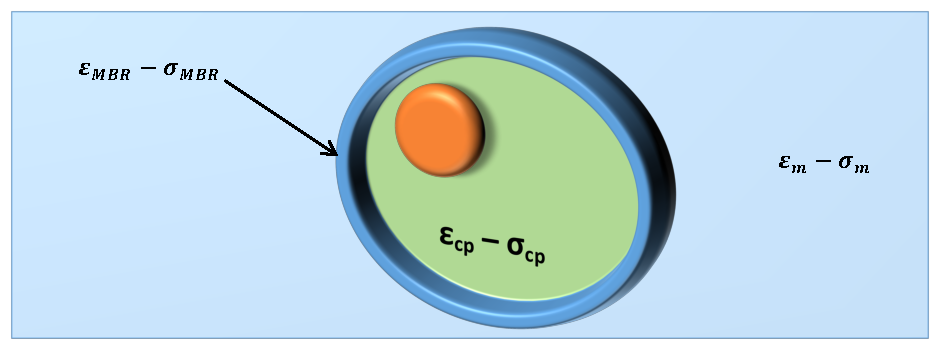
\includegraphics[width=0.8\textwidth,keepaspectratio, trim={0cm 0cm 0cm 0cm},clip]{figure1}    
	\caption[Cell permeability and conductivity distribution]{Representation of a cell with its electric characteristics. Internal cytoplasm characteristic permittivity $\epsilon_{cp}$ and conductivity $\rho_{cp}$. Extracellular fluid permittivity $\epsilon_m$ and conductivity $\rho_m$). Membrane permittivity described as ($\epsilon_{MBR}$) and conductivity ($\rho_{MBR}$).}
	\label{fig:cell}
\end{figure}

A cell can change its internal cytoplasm by two different means, either changing the permeability of their bilayer lipid membrane (BLM) or by using ionic channels or pumps. The BLM is about \SI{7}{\nano\meter} thick. By altering its permeability it allows lipids and water molecules to pass through~\cite{ivorra2003bioimpedance}. The interface between the extracellular space, the cell membrane and intracellular space ($\rho_m \rightarrow \rho_{MBR} \leftarrow \rho_{cp}$) behaves as a capacitor. This is because the membrane is a dielectric between two conductors, which is represented as $C_m$ in figure \ref{fig:cell model}.

In contrast, parallel to BLM the ionic channels and pumps enhance membrane’s functionality. Ionic channels or “channel proteins” allow transport and exchange of certain types of ions such as $Na^{+}$, $K^{+}$, Chloride ($Cl^{-}$) and Calcium ($Ca^{2+}$) between the inside and outside of the cell~\cite{lvovich2012impedance}. Ion pumps are caused by sensitivity of the membrane to a voltage and are responsible for the membrane’s non–linear properties to low voltage. This pump causes cell polarisation that permits the flow of ion charges in the body. Electrically, these channels act as a resistor ($R_m$).

\begin{figure*}[!htbp]
	\centering
	\begin{subfigure}[t]{0.48\textwidth}
		\centering
		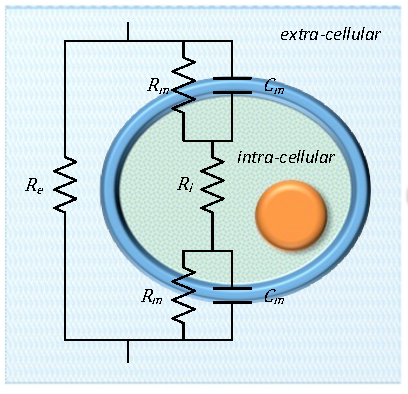
\includegraphics[height=6.5cm]{figure2a}
		\caption{Cell's equivalent circuit model}
		\label{fig:cell model}
	\end{subfigure}%
	~ 
	\begin{subfigure}[t]{0.48\textwidth}
		\centering
		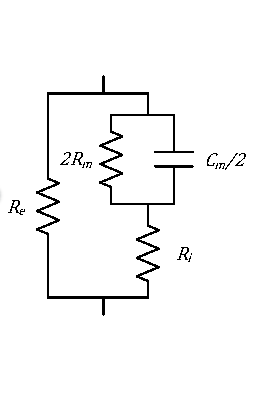
\includegraphics[height=6.5cm]{figure2b}
		\caption{Simplified circuit model}
		\label{fig:cell simp model}
	\end{subfigure}
	\caption[Electrical model of the cell]{Electrical model of the cell and its simplified version. $R_e$ is the resistivity of the extracellular medium, $R_i$ is the resistivity of the intracellular medium and $R_m$ and $C_m$ are the resistivity and capacitance of the membrane.}
	\label{fig:cell models}
\end{figure*}

According to previous analysis, the cell can be simplified in an equivalent electric circuit model as shown in Figure \ref{fig:cell models}. This model indicates that if AC is pumped into the extracellular medium, there are two possible paths for the current to go through. One way is around the cell which is represented by the resistive characteristic of the extracellular medium ($R_e$). In the second route, current flows through the cell. Indeed, AC may flow initially either over the BLM which is represented as a capacitance ($C_m$) or across ionic channels ($R_m$). Once in the cell, current travels via the intracellular medium ($R_i$) that is mostly resistive. Finally, the electrical current leaves the cell through the membrane, which it is again the same $C_m$ and $R_m$.

Since $C_m$ and $R_m$ have the same values when the current enters and exits the cell, this can be simplified in the electric model as two resistors in series ($2R_m$) and two capacitances in parallel ($C_m/2$) as can be seen in figure \ref{fig:cell simp model}.

When an EM field is applied to the tissue, cells respond according to the frequency applied showing three distinctive areas in the spectrum as described by Schawn et al.~\cite{schwan1957electrical,schwan1962electrical}. Figure \ref{fig:ABG dispersion} displays the dielectric response against frequency, which reveals valuable information about the functional and structural properties of the cell~\cite{lvovich2012impedance}. According to the graph, there are three denominating areas $\alpha$, $\beta$ and $\gamma$ dispersion. Firstly, $\alpha$ dispersion (from \SI{10}{\hertz} to a few \si{\kilo\hertz}) is generally associated with frequency dependent properties of the cells’ membrane. Secondly, $\beta$ dispersion (\SI{10}{\kilo\hertz} to several \si{\mega\hertz}) is related to the dielectric property of the cell membrane and the interaction between the internal and external mediums. Finally, $\gamma$ dispersion (> \SI{10}{\giga\hertz}) is due to dielectric relaxation of bulk dispersing media, the Debye dispersion in water (\SI{17}{\giga\hertz}) and the presence of small molecules. 

\begin{figure}[!htpb]
	\centering
	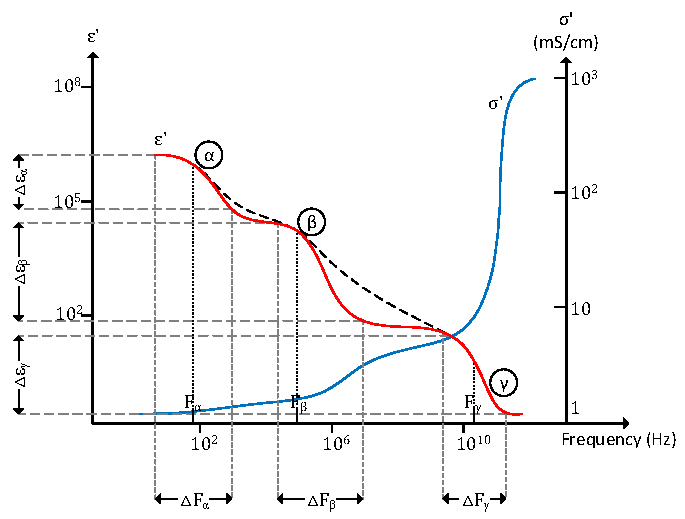
\includegraphics[width=0.8\textwidth,keepaspectratio, trim={0cm 1cm 0cm 0cm},clip]{figure3}    
	\caption[Alpha, Bet y Gama dispersion]{Representation of a cell with its electric characteristics. Internal cytoplasm characteristic permittivity $\epsilon_{cp}$ and conductivity $\rho_{cp}$. Extracellular fluid permittivity $\epsilon_m$ and conductivity $\rho_m$). Membrane permittivity described as ($\epsilon_{MBR}$) and conductivity ($\rho_{MBR}$).}
	\label{fig:ABG dispersion}
\end{figure}

In addition, the $\beta$ dispersion region provides supplementary information about the cell. Lvovich \cite{lvovich2012impedance} has divided this area into three subregions depending on the interaction of the electrical current with the cell. The $\beta_1$ relaxation is due to the capacitive membrane $C_m$, occurring in the low \si{\kilo\hertz} range. When the frequency is increased between \si{\kilo\hertz} and low \si{\mega\hertz} range, the internal cytoplasm of the cell can produce a $\beta_3$ dispersion because of a change from resistive to capacitive conduction. However, this capacitive component is often disregarded, simplifying the model into just a resistive element $R_i$. Ultimately, $\beta_2$ happens in the range of low \si{\mega\hertz} when the electrical charge movement through the cell shifts to a capacitive conduction.

This research document is centred in the $\beta$ dispersion region between \SIrange[scientific-notation = engineering]{100}{1000000}{\hertz}. The impedance plethysmography device designed described in chapter \ref{chapter design} is can operate in a different range of programmable frequencies up to \SI{100}{\kHz}. 

The ideal electrical model of the cell shown in figure \ref{fig:cell models} is a very close approximation that allows predicting bioelectrical impedance behaviour for dilute cell suspension. However, tissue is more complex than this simplified model because is composed by additional elements that need to be added to the analysis. For instance, tissue like muscle exhibits extreme anisotropy (conductivity is not the same when measured in different directions) \cite{lvovich2012impedance,dean2008electrical,foster1995dielectric}. Also, different resistivity values have been obtained when measuring bioelectrical impedance during the cardiac cycle longitudinally and transversally \cite{steendijk1993four}. Another example of how impedance changes with tissues properties can be seen in the performed by Casas et al. \cite{casas1999vivo}. This study showed differences between normal and ischemic tissue of a pig's myocardium muscle. Impedance clearly presented a different impedimetric response when a frequency sweep was done between \SIrange[scientific-notation = engineering]{10}{1000000}{\hertz}. 

\subsection{Mathematical representation of electrical impedance}
Electrical impedance can have a different response according to the frequency used. In a bioelectrical impedance analysis (BIA) the impedimetric response has to be represented as a function of the frequencies used and the magnitude and phase obtained. Different mathematical models have been studied based on the ideal and basic framework shown in figure \ref{fig:cell simp model}. Still, this model does not entirely represent the effect of the membrane at high frequencies. Debye produced the following equation that took into account suspension of free poles \cite{bertemes2002tissue}.

\begin{align}
\label{eq:Debye}
\varepsilon_r^* = \varepsilon_{HF} + \frac{\varepsilon_{LF} - \varepsilon_{HF}}{1 + j \omega \tau}
\end{align}

In this equation, $\varepsilon_r^*$ is the complex relative permeability, $\varepsilon_{LF}$ and $\varepsilon_{HF}$ represents permeability at low and high frequency respectively and $\tau$ is the relaxation time constant. For the other terms, $j \omega =2 \pi$ indicates the angular frequency in radians. However, it was not until 1941 when Cole brothers with their empirical work took into account dispersion by including in the Debye equation an additional parameter called $\alpha$, resulting in the equation \ref{eq:cole cole}. Presently, this mathematical formula is widely used to get the approximate value of impedance when taking biomedical measurements \cite{cole1941dispersion}.

\begin{align}
\label{eq:cole cole}
\varepsilon_r^* = \varepsilon_{HF} + \frac{\varepsilon_{LF} - \varepsilon_{HF}}{(1 + j \omega \tau)^{1-\alpha}}
\end{align}

The parameter $\alpha$ is limited for values between 0 and 1. When its value is equal to zero, the Cole-Cole equation will give the Debye equation (\ref{eq:Debye}) as a solution for polar dielectrics. Consequently, from this mathematical statement, it is possible to obtain data representation known as the Cole-Cole plot. That is a two-dimensional graph where the plot of $\varepsilon \prime\prime$ or the imaginary part of the equation is in the $y$-axis vs $\varepsilon \prime$ in the $x$-axis which is the real part of the solution. 

The representation of data using Cole-Cole representation allows to see changes in frequency for different tissues. This information is valid when spectroscopy studies are being performed. Regarding the most suitable frequency to measure impedance plethysmography, whole body bioelectrical impedance analysis has shown that limbs contributed significantly to the impedance at frequencies \SIlist{0.5; 50; 100}{\kHz} \cite{bracco1996segmental}. Therefore, any AC with this frequency spectrum is suitable for an impedance plethysmography instrument. 

%********************************** % Fifth Section  *************************************
\section{Bioelectrical impedance state of the art} %Section - 3.5
\label{section impedance state art}
Either a bioimpedance device or impedance plethysmography device operates under the principles described before. However, there are different alternatives to circuits and methods to measure impedance from the human body.  

Currently, there are efforts to implement impedance into wearable technology. For instance, Samsung Electronics released a hand-wrist size wearable device called simband~\cite{simsense}. In their product announcement, Samsung uses electrical impedance to measure the galvanic impedance response (GSR) and Bio-Impedance (Bio-Z). In figure \ref{fig:simsense} shows the actual sensor band (simsense), in its second generation counts with different sensors apart from the ones previously mentioned. Such as electrocardiogram signals (ECG), photoplethysmography (PPG), accelerometers and skin temperature. Nevertheless, this kind of device falls into the research spectrum and is still under development.

\begin{figure}[!htpb]
	\centering
	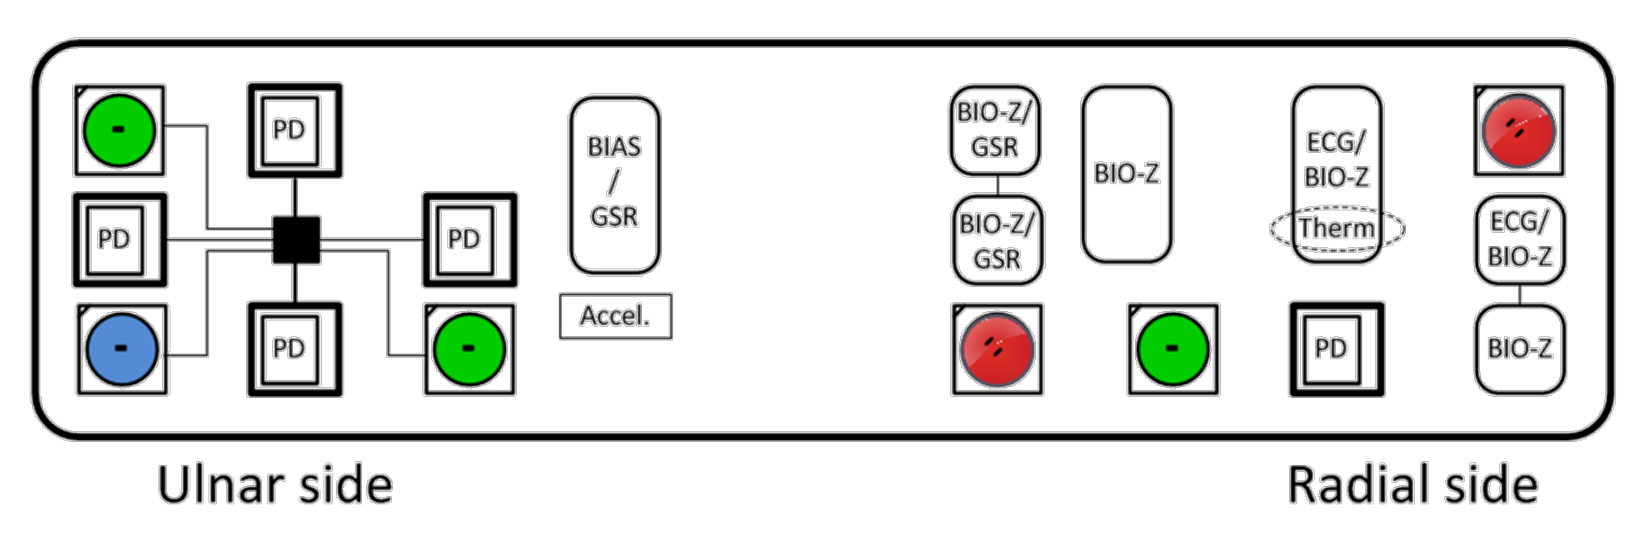
\includegraphics[width=8cm,keepaspectratio]{figure10}    
	\caption[\nth{2} generation Simsense board for the Simband]{\nth{2} generation Simsense board for the Simband. Image from \cite{simsense}}
	\label{fig:simsense}
\end{figure}

However, there are a significant number of devices that uses bioimpedance for different medical applications, such as impedance cardiography (ICG) devices. This kind of devices has been developed to measure different properties of the heart such as stroke volume (SV), cardiac output (CO) and systematic vascular resistance (SVR)~\cite{neath2005utility}.  Nevertheless, apart from its main application, this instrument has also been used to measure other medical parameters like proximal vein thrombosis (PVT)~\cite{hull1978impedance} or to measure levels of ischemia during orthopaedic surgery~\cite{distefano1973bioelectrical}.

Some companies are also working on creating alternative medical applications for bioelectrical impedance technology. One example of this is Australian company ImpediMed~\cite{impedimed} which own patents for this technology and have manufactured commercial devices approved by FDA focused on detecting body fluid contents in 3 different areas: Lymphedema product line designed to detect lymphatic obstruction conducting to inflammation and liquid retention.  Fluid Status/Body Composition product line intended to measure the content of water and fat in the human body. At last is their BMI research product, which has been created to calculate body mass index (BMI) using bioelectrical impedance analysis.

Another company that successfully has a FDA approved medical device using bioelectrical impedance in the market is Cheetah Medical \cite{cheetah} from Israel. This company based in Boston U.S. has remarkably developed a product to measure haemodynamics non-invasive using four electrodes configuration. The device is used in different hospital areas such as in critical care, haemodialysis, emergency department and operating theatres.

Next is Tanita Corporation, a Japanese company pioneer in the production of digital weight scales capable of performing a whole body composition analysis using either bioelectrical spectroscopy analysis or segmental bioelectrical impedance methods~\cite{tanita}. Moreover, their products are FDA approved and can provide an enormous number of readings from the human body including extracellular water content (EWC), intracellular water content (IWC), muscle balance, segmental analysis of muscle mass and fat percentage.

At last is the German company medis (Medizinische Messtechnik GmbH) which is a spin-off company from Institute of Biomedical Engineering of the Technical University Ilmenau. They manufacture medical equipment for cardiovascular diagnosis including impedance cardiographs and impedance plethysmography devices. However, their devices also combined other methods such as PPG and ECG to obtain a better assessment of the haemodynamics. 

\section{Basic components of a bioelectrical impedance device}
\label{section impedance basic}
It is evident that there are several number of medical devices using either biomedical or bioelectrical impedance technology. Nonetheless, regardless of the application most of the instruments include in their design the block diagram shown in figure \ref{fig:block diagram bioimpedance} within their designs. 

\begin{figure}[!htpb]
	\centering
	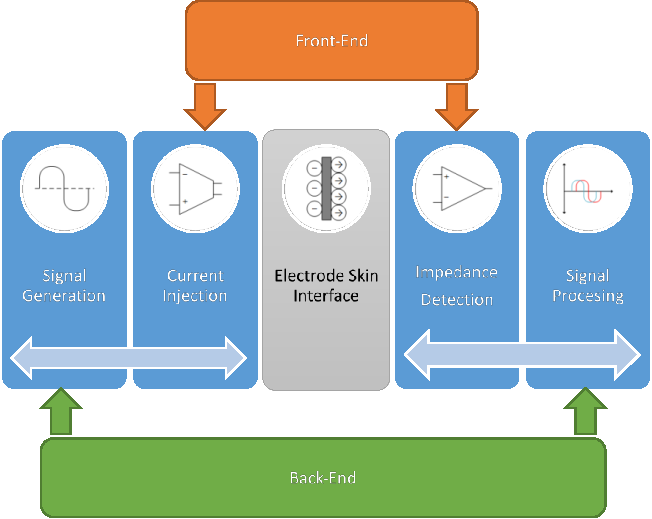
\includegraphics[width=9cm,keepaspectratio]{figure11}    
	\caption[Block diagram of a common bioimpedance device]{An bioimpedance device requires front-end and back-end components in order to detect changes of impedance efficiently.}
	\label{fig:block diagram bioimpedance}
\end{figure}

An impedance system can be divided into three different blocks: the first one called back–end commonly consists of the signal generation and digital analysis circuits to evaluate the signal sensed. Next is the front–end block that is comprised of all the circuitry before the contact with the skin such as current injection and signal detection electronics. Ultimately, skin electrode interface that behaves as an electronic circuit described in section \ref{section impedance electrodes}. 

Besides the back–end block is divided into two different sections. First signal generation circuits that depend on either extremely precise oscillators or Digital Signal Synthesizers (DDS) to generate accurate signal waves in a wide bandwidth with highly accurate amplitudes. The frequency exactness of these electronic circuits could be up to \SI{0.1}{\percent} \cite{ad:AD5930}.  Different kind of waveforms may be applied, but the most common one is a sinusoidal wave. 

In the other extreme is the signal processing circuits, used to evaluate signal’s amplitude and phase sensed by the front–end block.  As a matter of fact, powerful processors or microprocessors are used to digitalize and analyse the signals identified. Moreover, modern devices are also aided by advanced either Digital Signal Processors (DSP) or high–speed analogue to digital converters (ADC) capable of oversampling the signals detected. This kind of high precision and high–speed processors and chips are highly specialised and expensive.

Likewise, the front–end is also divided into two different sections current injection and signal detection circuits. The current injection circuit, as its name indicates, it is in charge of transferring the signal coming from the wave generator into the electrodes; some of the characteristics of these circuits are high bandwidth, accuracy and linearity. 

On the other hand, signal detection circuits receive the signal after this has passed through the sample under test. In contrast with specialised digital circuitry used on the back–end, the front–end mostly relies in highly precise analogue systems. These circuits can be implemented with either discrete components or custom chips. However, discrete components may have a limited response when bandwidths in the order of Megahertz is required. Consequently, custom microchip design containing current injection and sensing circuits are a better option because it reduces the influence of stray capacitances. 

\subsection{Methods of measuring bioelectrical impedance}
\label{section impedance state art.1}
Some authors have called bioelectrical impedance analysis (BIA) the method to interpret impedance measurements from the human body \cite{kyle2004bioelectrical}. Different techniques have been developed using a single or multiple frequencies and a different amount of electrodes. This section describes the most common form of BIA techniques available explaining their operation frequency, electrodes location and data representation.

\subsubsection{Single Frequency BIA}
Single frequency bioimpedance analysis uses a single frequency to perform whole body’s impedance analysis. The most common frequency used for this purpose is \SI{50}{\kilo\hertz}, used mostly for body composition analysis where current flows through the entire body applying electrodes on the hands and feet in a tetrapolar set up as displayed in Figure \ref{fig:single f BIA}. This method can provide an approach to whole body composition analysis, including free–fat mass (FFM) and a weighted sum of ECW and ICW resistivities \cite{kyle2004bioelectrical}. Nonetheless, measurements can be notably affected by the subject’s hydration level \cite{gudivaka1999single,schoeller2000bioelectrical}.

\begin{figure}[!htpb]
	\centering
	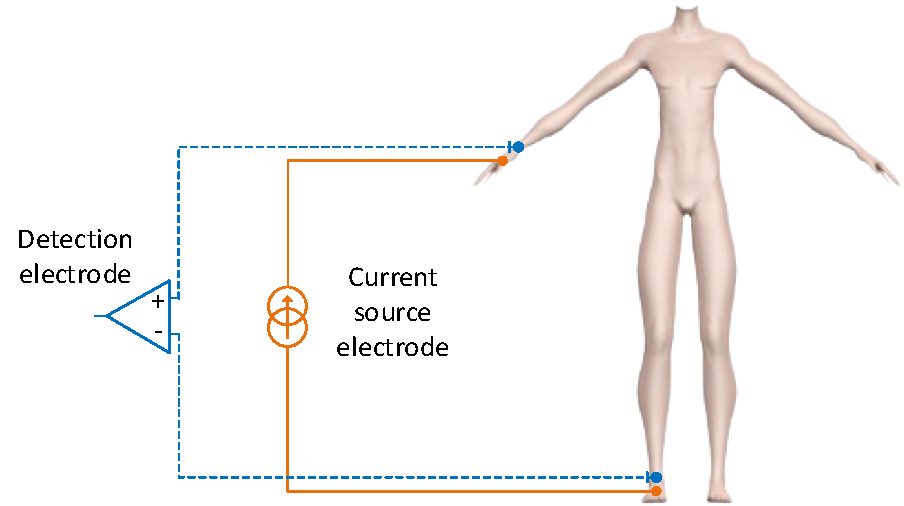
\includegraphics[width=0.7\textwidth,keepaspectratio]{figure12}    
	\caption[Common electrodes placement for whole body BIA and BIS]{Common electrode location for single frequency BIA, multi–frequency BIA and BIS (Adapted from Kyle \cite{kyle2004bioelectrical})}
	\label{fig:single f BIA}
\end{figure}

\subsubsection{Multi–frequency BIA}
This method is very similar to the one described previously; it also focuses on whole body analysis. Even though this technique uses empirical linear regression models and multiple set frequencies to evaluate total body water (TBW), FFM, ICW and ECW. Likewise, it has been effective as a tool to assess amyotrophic lateral sclerosis (ALS) \cite{wang2011electrical}. The most common frequencies used are \SIlist{1;5;50;100;200;500}{\kilo\hertz} \cite{kyle2004bioelectrical}. 

However, some studies have revealed that there is a poor reproducibility in frequencies below \SI{5}{\kilo\hertz} and above \SI{200}{\kilo\hertz}. Also, multi–frequency BIA has some improvements compared to single frequency BIA when measuring similar parameters in the body but they are not clinically significant \cite{hannan1995comparison}. Last, single frequency BIA is more accurate to calculate TBW in critically ill subjects, whereas multi–frequency BIA is more accurate and less biased predicting ECW \cite{patel1996estimation}. 

\subsubsection{Bioelectrical impedance spectroscopy (BIS)}
Although multi–frequency BIA and BIS use a broad range of frequencies, BIS uses mathematical analysis and a mixture of equations to find the whole body’s equivalent impedance. One of these mathematical analysis’ is the implementation of the Cole–Cole \cite{cole1941dispersion} calculation as shown in Equation \ref{eq:cole cole} and mixing theory model from Hanai \cite{hanai1968electrical}. From these models, it is possible to predict and, which can provide information about TBW and ECW \cite{hanai1968electrical}. 

For this method to work properly, it has to use mathematical models, constants and equations obtained from a healthy population \cite{patel1994estimation}. If this technique needs to be utilised for a specific purpose or population, such as monitoring a disease, either a new calibration or a different mathematical model must be applied to get a closer correlation between the results obtained, and the ones predicted \cite{schoeller2000bioelectrical, de1997predicting}. However, the use of mixture methods has shown combined results, some of them being accurate, with others showing no improvement or even worse results compared to previous techniques using regression approaches \cite{kyle2004bioelectrical}. The use of BIS can be adequate and more accurate if previous data is known to fit the better curve to the results. As a result, some researchers have implemented the use of neural networks to try to predict results according to previous readings \cite{songer2001tissue,kun2003algorithm}. 

\subsubsection{Segmental bioelectrical impedance analysis}
This method requires applying two additional electrodes in other parts of the body such as opposite wrist and foot, wrist and shoulder, upper iliac spine and ankle, proximal part of the forearm and lower leg, and shoulder and upper thigh. However, there is no standardisation in the position of the electrodes, which might result in different current distribution for the whole body measurements \cite{kyle2004bioelectrical, woodrow1996segmental}. There is a good correlation between appendicular lean body mass evaluated by X–ray absorptiometry (DXA) and segmental BIA adjusted by stature, at all frequencies. It also showed that upper extremities constitute the main component of impedance at high frequencies (order of \si{\kHz}) because there is a higher content of fat in arms than in legs \cite{delorenzo2003segmental}. 

However, it has been recommended not to be used this method in healthy young adults as lacks of accuracy \cite{laforgia2008body,leahy2012comparison}. Calculating TBW requires measuring the length of the body segments (arm, trunk and leg) in order to make calculations for the analysis but Thomas et al. [44] considers that this extra effort is not justified when similar outputs can be obtained with BIA method. In contrast, segmental BIA has been found useful in the in the calculation of fluid distribution in some illnesses such as ascites (abnormal accumulation fluid in the abdominal cavity) and during surgery \cite{kyle2004bioelectrical}. Moreover, it is very practical for patients with renal failure, where and imbalance of fluids can be detected more accurately \cite{woodrow1996segmental,thomas2003comparison}. 

\subsubsection{Localised bioelectrical impedance analysis}
All the previous methods are focused on whole body measurements. On the other hand, localised BIA aims to avoid the incidence of the effects of different variables such as hydration, fat fraction, geometry boundary conditions, etc. According to this focusing in well–defined segments of the body allows minimising the effect of those variables. Moreover, when the segment is confined into a small volume such small segment is possible to calculate blood flow or plethysmography. The use of four electrodes is critical for this kind of applications because it creates the boundaries of the system. 

The calculation of the BIA also simplifies because empirical regression models according to the population can be applied \cite{kyle2004bioelectrical}. In some cases is required to get dimensions of the limb of interest to obtain its geometric volume for a more detailed calculation.  Some of the cases where this technique has been applied are the analysis of limb ischemia \cite{songer2001tissue,kun1994tissue} breast cancer \cite{zou2003review}, detection and monitoring of Lymphedema \cite{vicini2012bioelectrical} and local abdominal fat mass \cite{scharfetter2001assessing} just to name some. 

\subsubsection{Bioelectrical impedance vector analysis}
This method developed by Piccoli et al. \cite{piccoli2000relationship, piccoli2002impedance} at the beginning of 2000’s assesses fluid body volume through patterns of vector distribution based on resistance ($R$) and admittance ($X_{c}$) values \cite{thomas2003comparison}. Furthermore, on top of those values, BIVA requires height and genre from the patient so as to establish a statistical ranking compared to similar population (reference population). 

\begin{figure}[!htpb]
	\centering
	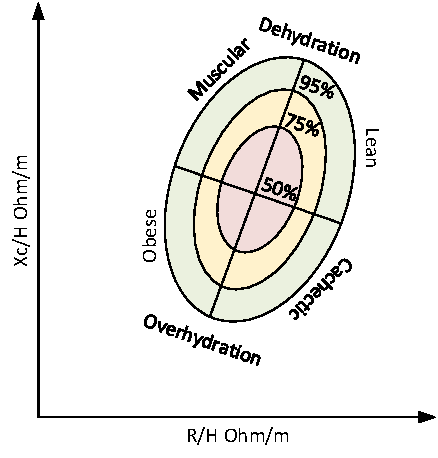
\includegraphics[width=0.4\textwidth,keepaspectratio]{figure13}    
	\caption[BIVA representation]{BIVA representing the vector distribution based on resistance and admittance}
	\label{fig:BIVA plot}
\end{figure}

Data is represented in a graph $R$ vs. $X_{c}$, comparing subject’s data to ellipses tolerances from reference population at \SIlist{50;75;95}{\hertz} previously calculated in a healthy population of the same race, the age and sex \cite{kyle2004bioelectrical,piccoli2000relationship, piccoli2002impedance}. As an illustration, if a measurement taken falls below \SI{75}{\percent} on the left of right of the ellipse then it can indicate an anomaly in tissue’s impedance. This data can be interpreted as changes in tissue hydration and more or less body cell mass (BCM) in lean body tissue. BIVA has been validated for different medical instances for the management of body hydration such as in acute heart failure, haemodialysis, hydration, diuresis, ultrafiltration and body hydration in emergency room \cite{disomma2011consensus}. 

%********************************** %First Section  **************************************
\section{The principle of bioelectrical impedance plethysmography} 
\label{section iPG principle}
As previously described in section \ref{section literature BI}, iPG is the measurement of volume changes through the equivalent impedance of a human body part \cite{corciova2011peripheral}. Indeed, when heart’s systole increases blood flow, the volume of a limb rises due to the inflow of arterial blood (swelling) \cite{martinsen2011bioimpedance}. Consequently, there are changes of impedance correlated to the changes of volume and flow in any part of the body. Some of the medical applications of this technology include measurement of heart stroke volume (SV), cardiac output (CO), thoracic respiratory volume, oedema and detection of deep vein thrombosis (DVT)~\cite{holohan1996plethysmography}.  

The genesis of impedance plethysmography can be traced back to the model proposed by Jan Nyober~\cite{nyober1950electrical}. The author describes extremities as cylinders, where an inner cylinder represents a blood vessel, and the outermost is the surrounding tissue. The whole electrical conductance path is resulting from the sum of the parallel conductance of blood and tissue within a segment. In fact, this theory called parallel conductor was later confirmed by the experiments performed by Shimazu et al. \cite{shimazu1982evaluation}. There have been some doubts about how much is blood's impedance contribution to the total impedance signal. Nonetheless, it has been demonstrated through in-vitro experiment that blood (haematocrit = $ 26 \pm 4 \%$) contributed to \SI{10}{\percent} of the impedance signal. In the study, the final result was obtained when comparing the measurements of a saline buffer solution and blood in extensible arteries and rigid tubes~\cite{peura1978influence}.

\begin{figure}[!htpb]
	\centering
	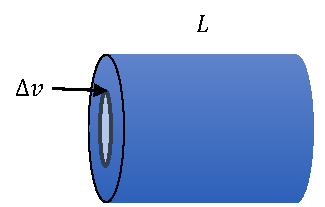
\includegraphics[width=5.5cm,keepaspectratio]{figure5}    
	\caption[Two compartment cylinder model]{Two compartment cylinder model of length L and parallel volume increment}
	\label{fig:two cylinder model}
\end{figure} 

In principle, recurring to the anatomy described in the section \ref{section literature anatomy}, the normal volume ($V$) of a human forearm contain within a certain length $L$ is given the bones, muscle, fat and blood structure around a cross-sectional area ($A$) (see figure \ref{fig:two cylinder model}). When a circulatory cycle takes place, an additional amount of blood enters to the limb through the brachial artery, increasing the total volume of the limb in $\Delta V$. Thus, the new limb's total volume at the peak of the systole will be equivalent to $V + \Delta V$. As a result, a shunting impedance $Z_b$ is produced given by the following equation \cite{swanson1976origin, webster2009medical}:

\begin{align}
	\label{eq:blood impedance}
	Z_b = \rho_b \frac{L}{\Delta A}
\end{align}

where $\rho_b$ is the blood's conductivity and $\Delta A$ is the increase of the cross-sectional area of the limb. However, for this formula to works, some assumptions must be taken into account: the arterial expansion is uniform along the tissue, the blood resistivity ($\rho$) is constant, and the flow of current is parallel to the artery \cite{bera2014bioelectrical}. Therefore, the artery volume change can be obtained with the following formula \cite{swanson1976origin, webster2009medical}.

\begin{align}
	\label{eq:delta volume}
	\Delta V = L \times \Delta A = \rho_b \frac{L^2}{\Delta A}
\end{align}

As it can be noticed from the previous equation, during the cardiac cycle the area of the artery increases from $A$ to $A + \Delta A$. However, the impedance of $Z_b$ is also affected by the additional impedance ($\Delta Z$) produced by the increment $\Delta A$, and this $Z_b$ is connected in parallel to $Z$. Therefore, Nyober \cite{nyober1950electrical} proposed that the practical parallel resistive value of the displaced blood can be originated from the parallel relation between the initial base resistance and the new resistance value, given by the following expression:

\begin{align}
	\label{eq:parallel model}
	\Delta Z = (Z_b \parallel Z) - Z = \frac{Z^2}{Z + Z_b}
\end{align}

where $Z$ is equivalent to the limb's original resistance at diastole and $Z_b$ represents the increase of new total resistance. Now, as $Z_b \gg Z$, then $Z_b$ can be rewritten as:

\begin{align}
	\label{eq:parallel model2}
	\frac{1}{Z_b}\cong -\frac{\Delta Z}{Z^2}
\end{align}

Finally, the change in the limb volume in association with the variation of impedance can be expressed by the equation \ref{eq:nyober dV}. It must be noted that the negative sign is an indication of direction.

\begin{align}
	\label{eq:nyober dV}
	\Delta V = -\rho_b \frac{L^2}{Z^2}\Delta Z
\end{align}

Different equations aroused complementing the Nyboer's work. One of this modifications is the Kubicek et al. method~\cite{karnegis1966development, kubicek1970impedance, kubicek1979impedance}. His equation is widely used especially when measurements from the measurement of impedance cardiography from the thoracic box and to deduct stroke volume of the heart. Other, popular work is the contribution done by Sramek~\cite{sramek1986bomed}. The author also modified Kubicek's equation eliminating the dependence $L$ and $\rho_b$,  and introduced a constant obtained from statistical methods named "volume of electrical participating tissue". Alternative calculation methods have been developed using admittance instead of impedance.

Yamakoshi \cite{shimazu1982evaluation,yamakoshi1980limb,yamakoshi1978admittance} in his research and patent work uses impedance reciprocate, admittance $(Y=Z^{-1})$ to estimate blood flow using plethysmography which worked better with analogue computers of the time. In his work, the author states that the first gradient of the computation result to time is indicative of the blood rate in the limb being examined. However, the algorithms used in the present work will stick to the original equations proposed by Nyober.

\subsection{Two or four electrode measurements}
\label{section iPG electrodes}
There are various electrode topologies to take impedance measurements. Some of the options include two-electrode, three electrode and four electrode setting. The following analysis describes the difference between the two most common option bipolar and tetrapolar electrodes.

As described in section \ref{section impedance electrodes}, the circuit model of an electrode is equivalent to a charge transfer resistance ($R_{CT}$) in parallel to an unknown interface's impedance ($Z_{CPE}$), these two components represent the impedance and polarization of the electrode-electrolyte interface \cite{neuman2000biomedical}. Then, in series with a the tissue impedance ($Z_t$) \cite{lvovich2012impedance}. Completing this model also requires to include the half-cell potential, which is represented as a battery ($E_{hc}$) \cite{neuman2000biomedical}. Therefore, the complete electrode model can be modeled as the one shown in figure \ref{fig:electrode model}.

\begin{figure}[!htpb]
	\centering
	\begin{circuitikz}
		\draw[american](0,0) 
		to[battery=$E_{hc}$] (2,0)
		to[short, o-*] (2,0) -- (2,1)
		to[generic=$Z_{CPE}$] (4,1) -- (4,0)
		to[short, o-*] (4,0)
		to[generic=$Z_t$] (6,0)
		(2,0) -- (2,-1)
		to[R=$R_{CT}$](4,-1)--(4,0)
		;
	\end{circuitikz}
	\caption[Electrode equivalent circuit]{The electrical model of an electrode is equivalent to a battery that represents the half-cell potential, }
	\label{fig:electrode model}
\end{figure}

The most common option to measure impedance in the body is the tetrapolar option. The following analysis shows the ideal cases when using two and four electrodes in the measurements.

\subsubsection{Bipolar electrode measurement}
The bipolar electrodes method uses the same pair of electrodes for current injection and measurements. The figure \ref{fig:bipolar} shows the connection and the simplified circuit model of the set-up. As it can be noticed, the current $I$ is in the path of the circuit $Z_{C1} - Z_t - Z_{C2}$. Therefore, there is a potential drop on the electrodes, and the total measurement includes the tissue potential plus the electrodes. 

\begin{figure}[!htbp]
	\centering
	\begin{subfigure}[b]{0.48\textwidth}
		\centering        
		\begin{circuitikz}[scale=0.9]
			\fill[black!40!white] (0,0) rectangle (1,0.5);
			\fill[black!40!white] (3,0) rectangle (4,0.5);
			\fill[red!40!white] (-1,0) rectangle (5,-0.25);
			\node[text width=1cm] at (2.05,-0.5) {Skin};
			\node[text width=1.8cm] at (2.05,0.8) {Electrodes};
			%    \draw[arrow] (2.05,0.8) -- (1.05,0.5);
			
			\draw
			(3.5,2.5)to[sI=$I$](0.5,2.5)--(0.5,4)
			to[voltmeter](3.5,4)--(3.5,2.5)
			(0.5,4)--(0.5,0.5)
			(3.5,4)--(3.5,0.5)
			;
			
		\end{circuitikz}
		\caption[Bipolar electrodes position]{Simplified circuit model of the bipolar electrodes position. The current driving are the same as the potential sensing.}
		\label{fig:bipolar conection}
	\end{subfigure}%
	~
	\begin{subfigure}[b]{0.48\textwidth}
		\centering    
		\begin{circuitikz}[american]
			\draw (0,0) 
			to[generic=$Z_{C1}$, i<=$I$](0,3)
			(0,4)to[battery=$E_{h1}$](0,3)
			(0,4)--(0,4.5)
			to[short, -*](0,4.5)
			(3,4.5)to[sI=$I$]
			(0,4.5)--(0,6)
			to[voltmeter](3,6)--(3,4.5)
			to[short, -*](3,4.5)--(3,4)
			to[battery=$E_{h2}$](3,3)
			to[generic=$Z_{C2}$, i<=$I$](3,0)
			to[generic=$Z_{t}$, i<=$I$](0,0)
			;
		\end{circuitikz}
		\caption[Simplified model of bipolar electrodes position]{Simplified circuit model of the bipolar electrodes position.}
		\label{fig:bipolar circuit}
	\end{subfigure}
	\caption[Bipolar electrodes position and equivalent circuit]{Bipolar electrodes position in a measurement over the skin with the equivalent circuit. The current driving is the same as the potential sensing. $Z_{c}$ represents the impedance of the electrodes and $Z_t$ is equivalent to the body's impedance.}
	\label{fig:bipolar}
\end{figure}

The unknown impedance added by the electrodes can be proof when analysing the current path of the equivalent circuit in figure \ref{fig:bipolar circuit}. From there it can be seen that the potential ($V$) measured is equal to the equation \ref{eq:bipolar}.

\begin{equation}
	\label{eq:bipolar}
	V = E_{h1} + (Z_{C1}+Z_t+Z_{C2})I - E_{h2}
\end{equation}  

Then for a current $Ie^{j \omega t}$ the voltage drop for the whole network is equivalent to equation \ref{eq:bipolar2}. If it is considered that the half-potential cell is the same on each electrode, then these terms cancel out. 

\begin{gather}
	\label{eq:bipolar2}
	V(t) = \cancel{E_{h1}} - \cancel{E_{h2}} + Z_{C1}I e^{j \omega t} +Z_t I e^{j \omega t} +Z_{C2}I e^{j \omega t}
	\\
	\label{eq:bipolar3}
	V(t) = Z_{C1}e^{j \omega t} +Z_t I e^{j \omega t} +Z_{C2}I e^{j \omega t}
\end{gather}

From section \ref{section impedance principle} can be remembered that the voltage produced by an impedance is complex. Therefore, there is a phase shift for each of the impedance of the network denoted as $\theta$.

\begin{equation}
	\label{eq:bipolar4}
	V(t) = V_{C1} e^{j(\omega t + \theta_1)} + V_t e^{j( \omega t + \theta)} +V_{C2} e^{(j \omega t + \theta_2)}
\end{equation} 

Finally, with equation \ref{eq:ohm} is possible to calculate the impedance of the whole network.

\begin{gather}
	\label{eq:bipolar5}
	Z_m(t) =\frac{V(t)}{I(t)} = \frac{V_{C1} e^{j( \omega t + \theta_1)} + V_t e^{j( \omega t + \theta)} +V_{C2} e^{(j \omega t + \theta_2)}}{I e^{j \omega t}} \\
	Z_m(t) = Z_{C1}e^{j\theta_1} + Z_{t}e^{j\theta} + Z_{C2}e^{j\theta_2}
\end{gather} 

As it can be noticed, the final measurement ($Z_m(t)$) in a bipolar technique includes the complex impedance of the electrodes. This unknown impedance results in a significant error added to the total measure. If the impedance of the electrodes were more significant than the one of the skin, this completely hides the real value of the tissue's impedance. For this reason, a bipolar configuration is not the best option for bioelectrical impedance measurements. 

\subsubsection{Tetrapolar electrode configuration}
The tetrapolar method is the most common method to measure bioelectrical impedance in the human limbs \cite{costeloe1980continuous, yamakoshi1980limb, nyboer1974blood, yamamoto1992impedance}. Some of the advantages of this method are that in theory cancels out the added impedance of the measuring electrodes. However, this can be achieved if follows these conditions: first, the input impedance of the measuring instrument is infinite, or in the best estimate the impedance is greater than the one from the body. Second, the contact area of the electrode with the skin surface is flat an even.

Currently, meeting this conditions can be quite hard to get but is possible to get close to them. Measuring impedance using state of the art of integrated circuits (IC) is likely to achieve high input impedance, in the order of \si{\giga\ohm} \cite{ad:AD8421}. Compared to hundreds of ohms of the soft tissue in humans \cite{faes1999electric, grimnes1983impedance}, the error is minimised dramatically. Additionally, the area of contact can be improved if electrodes with gel are uses because the result in lower skin impedances when the skin is wet \cite{mcadams1996factors, grimnes1983impedance}.

The figure \ref{fig:tetrapolar} shows the common electrode topology and the equivalent circuit. Usually, the outer pair is used for current injection and the internal for voltage measurement (see figure \ref{fig:tetrapolar electrodes}). The figure \ref{fig:tetrapolar circuit} shows the simplified equivalent circuit, which analysis will be performed to estimate the impedance contribution of electrode $Z_{C2}$ and $Z_{C4}$. 

\begin{figure}[!htbp]
	\centering
	\begin{subfigure}[H]{\textwidth}
		\centering    
		\begin{circuitikz}
			\fill[black!40!white] (0,0) rectangle (1,0.5);
			\fill[black!40!white] (1.5,0) rectangle (2.5,0.5);
			\fill[black!40!white] (3.5,0) rectangle (4.5,0.5);
			\fill[black!40!white] (5,0) rectangle (6,0.5);
			\fill[red!40!white] (-1,0) rectangle (7,-0.25);
			\node[text width=1cm] at (3.2,-0.5) {Skin};
			
			\node at (0.0,0.8) (E1){E1};
			\node at (1.5,0.8) (E2){E2};
			\node at (3.5,0.8) (E3){E3};
			\node at (5.0,0.8) (E4){E4};
			\draw
			(0.5,0.5)--(0.5,3.0) to[sI<=$I$]   (5.5,3.0)--(5.5,0.5)
			(2.0,0.5)--(2.0,1.5) to[voltmeter] (4.0,1.5)--(4.0,0.5)
			;
			
		\end{circuitikz}
		\caption[Tetrapolar electrode position]{Tetrapolar electrode position for most of bioelectrical impedance measurements. The outermost electrodes (E1 and E4) are connected to the AC source. The potential electrodes are connected to the inner electrodes (E2 - E3).}
		\label{fig:tetrapolar electrodes}.
		
	\end{subfigure}
	\\
	\begin{subfigure}[H]{\textwidth}
		\centering
		\begin{circuitikz}[american]
			\draw (0,0) 
			to[generic=$Z_{C1}$, i<=$I$](0,2)
			(0,4)to[battery=$E_{h1}$](0,2)
			(0,4)--(0,5)
			(6,5)to[sI=$I$](0,5)
			(6,5)--(6,4)
			to[battery=$E_{h2}$](6,2)
			to[generic=$Z_{C4}$, i<=$I$](6,0)
			to[generic=$Z_{t2}$, i<=$I$](4,0)
			to[generic=$Z_{t}$, *-*, i<=$I$](2,0)
			to[generic=$Z_{t1}$, i<=$I$](0,0)
			
			(2,0)to[generic=$Z_{C2}$, i=$I{=}0$](2,2)
			(2,4)to[battery=$E_{h1}$](2,2)
			(2,4)to[voltmeter](4,4)
			to[battery=$E_{h1}$](4,2)
			to[generic=$Z_{C3}$](4,0)
			;
		\end{circuitikz}
		\caption[Simplified electrical model of the tetrapolar electrodes model]{Simplified model of the tetrapolar electrodes model. $Z_C$ represents the impedance of the electrodes. $Z_b$ is the impedance of the body at each end of the electrodes. In an ideal setting, the voltmeter has infinite input impedance, therefore no current flows through the electrodes $Z_{c2}$ and $Z_{c3}$.}
		\label{fig:tetrapolar circuit}
	\end{subfigure} 
	\caption[Tetrapolar electrodes position and equivalent circuit]{Tetrapolar electrodes position in a measurement over the skin with the equivalent circuit.}
	\label{fig:tetrapolar}
\end{figure}    

Similarly, as the bipolar example, the current applied is equal to $I(t)=I e^{j \omega t}$. Thus, the potential drop around the section of the tissue being measured $Z_t$ will be equivalent to equation \ref{eq:tetrapolar}.

\begin{gather}
	\label{eq:tetrapolar}
	V(t) = Z_t I e^{j \omega t} \\
	\label{eq:tetrapolar2}
	V(t) = V_t e^{j (\omega t + \theta)}
\end{gather} 

In this case, because ideally the current flowing trough $Z_{C2}$ and $Z_{C3}$ is zero, the measured potential will be equivalent to the one from the body segment. Therefore, the final impedance $Z_m$ can be calculated using equation \ref{eq:tetrapolar3}.

\begin{gather}
	\label{eq:tetrapolar3}
	Z_m(t) = \frac{Z(t)}{I(t)} = \frac{V_t e^{j(\omega t + \theta)}}{I e^{j\omega t}} \\
	\label{eq:tetrapolar4}
	Z_m(t) = Z_t e^{j \theta}
\end{gather}

Finally, the measured impedance $Z_m$ is equivalent to the one complex impedance from the body segment $Z_t e^{j \theta}$, reducing the incidence of the potential electrodes. 

\subsection{Alternative applications of impedance plethysmography}
The plethysmography waveform is also utilised to quantify measurements of pulsatile volume, blood flow beat to beat, blood pressure and pulse wave velocity. In this case, the waveform is equivalent to the AC component of the impedance signal. The contribution of this signal to the total of the signal is between \SIrange{0.1}{1}{\percent} of the total of the signal. Sometimes, it is necessary to implement low noise techniques to picking up the signal hidden within the basal impedance. 

The most typical application of the waveform is the quantification of blood flow beat to beat. By applying Nyboer's equation to the waveform signal is also possible to quantify peak-peak blood volume and peak net inflow. For instance, the patent presented by Marks~\cite{marks1985computer} shows the application of quantifying blood flow in upper extremities by computing the derivatives of the waveform signal producing the results claimed. Another example, taking measurements from lower limbs is the work performed by Porter~\cite{porter1985measurement} where an impedance cardiograph was used to obtain the waveform signals and computed using Kubicek's equation \cite{karnegis1966development, kubicek1970impedance, kubicek1979impedance} and concluding the potential use of the signal to evaluate limb oedema. 

Another application of the waveform is the evaluation of blood pressure continuously. Blinov~\cite{blinov1997plethysmographic} demonstrated that pressure could be deducted if blood flow is known. As explained before, blood flow can be estimated beat-beat by deriving the waveform after applying Nyober's equation. As a result, the equation transforms into:

\begin{align}
\label{eq:dvdr}
dV = \rho \frac{L^2}{Z^2} dZ
\end{align}

Volume rate is defined as the change of volume in time. Then blood flow rate $(\dot{Q})$ is defined by the following equation:

\begin{align}
\label{eq:Q}
\dot{Q} = \frac{dV}{dt}=-\rho \frac{L^2}{Z^{2}} \frac{dZ}{dt}
\end{align}

where $W$ is the hydraulic resistance and $P$ is pressure. The hydraulic resistance is a function of the geometry of the artery given by radius $r$ and the viscosity of the blood $\mu$.

\begin{align}
W=\frac{8 l \mu}{\pi r^4}
\end{align}

Replacing equation $W$ into equation $\dot{Q}$ the pressure for a defined segment can be expressed by the following equation:

\begin{align}
P = -\frac{8 L \mu \pi}{\rho} \frac{dZ}{dt} = k \frac{dZ}{dt}
\end{align}

where $k$ is a constant value function of the distance between the electrodes, physiological constants of the blood at a particular measurement frequency. The sign in the equation just denotes that the changes in the resistance and pressure are opposite. Thus the sign can be disregarded while performing calculations.

Finally, the waveform obtained from impedance plethysmography can also be applied to evaluate pulse-wave velocity (PWV) in limbs. Measuring PWV can be accomplished by computing the time arrival difference between two reference measurement points and estimating the time difference between both waveforms. PWV is also an important indicator of deterioration in the cardiovascular system. This method requires two or more electrode arrays to measure the differential of electrical potential along a body segment. For its convince is easily applied to upper and lower limbs. This measurement technology has been successfully demonstrated by some researchers like Risacher et al~\cite{risacher1993impedance} where measurements were recorded using a multi-array electrode system. Some of the recommendations to the successful application of this method recommended by the author are taken special emphasis in the sensitivity to noise that this method may come across~\cite{risacher1992computation}, the use of high-precision and reproducible by the electrode array, accuracy in the measurement of the distance separating measuring sites, high sampling frequency to ensure higher accuracy in the calculation of time intervals. There are limits when recording these signals from a small body where location and geometry of the electrodes are prime for this application. It has been shown that is possible to record this signal from an area as small as \SI{1.5}{\cm} by \SI{7}{\cm} which also increases the possibility of portability~\cite{cho2009bio}. 



%********************************** % Sixth Section  *************************************
\section{Impedance plethysmography in the forearm}
\label{section impedance plethysmography}
As it has been noted, impedance plethysmography is capable of measuring the changes of blood in different parts of the body. Now in this section, it will describe more in depth how these changes occur in a limb. During the study described in this document, localised BIA is the most suitable method to estimate blood flow in the human body. The cylindrical shape of the forearm is a perfect place to measure impedance plethysmography. Also, its location provides valuable information about circulatory peripheral illnesses as described in chapter \ref{chapter background}.

Depending on the medical application an impedance plethysmography instrument (iPG) device can provide two type of signals, one dedicated to the basal impedance or the dynamic component. Both signal medical information about tissue health and also blood volume. Hence, one aim of this study is to design a device capable of providing both signals and the option of having an additional sensing channel for differential studies in the future.

There is not much variation from the structure of a bioimpedance device as shown in figure \ref{fig:block diagram bioimpedance} and an impedance plethysmography instrument. The electrodes are the first difference from a bioimpedance device. Commonly, circumferential band electrodes are used to take these measurements as shown by some studies \cite{ bera2014bioelectrical, mohapatra1979measurement, yamakoshi1980limb, porter1985measurement, corciova2011peripheral, anderson1984impedance}. However, some studies have shown that the there is not much difference when using single point electrodes such as ECG and band electrodes \cite{qu1986motion, sherwood1991comparison, patterson1991impedance}. In fact, these studies have shown that spot electrodes improve the signal-to-noise ratio enhancing the quality of the impedance measured. One reason for this is infection control, by using disposable ECG electrodes also limits cross-contamination in a clinical setting.

Bioimpedance measurements can be achieved with only two electrodes, but impedance plethysmography measurements commonly use four electrodes configurations. Most of the studies rely on tetra-polar electrodes set-up which is quite the norm for volume/flow measurements \cite{costeloe1980continuous, yamakoshi1980limb, nyboer1974blood, yamamoto1992impedance}. As shown by figure \ref{fig:tetrapolar iPG} a pair of electrodes placed at the outermost part of the segment are used to inject a high-frequency current. Whereas, the second pair of electrodes senses the voltage drop coming from the body segment. These sensing electrodes are arranged between the current electrodes. 

\begin{figure}[!htpb]
	\centering
	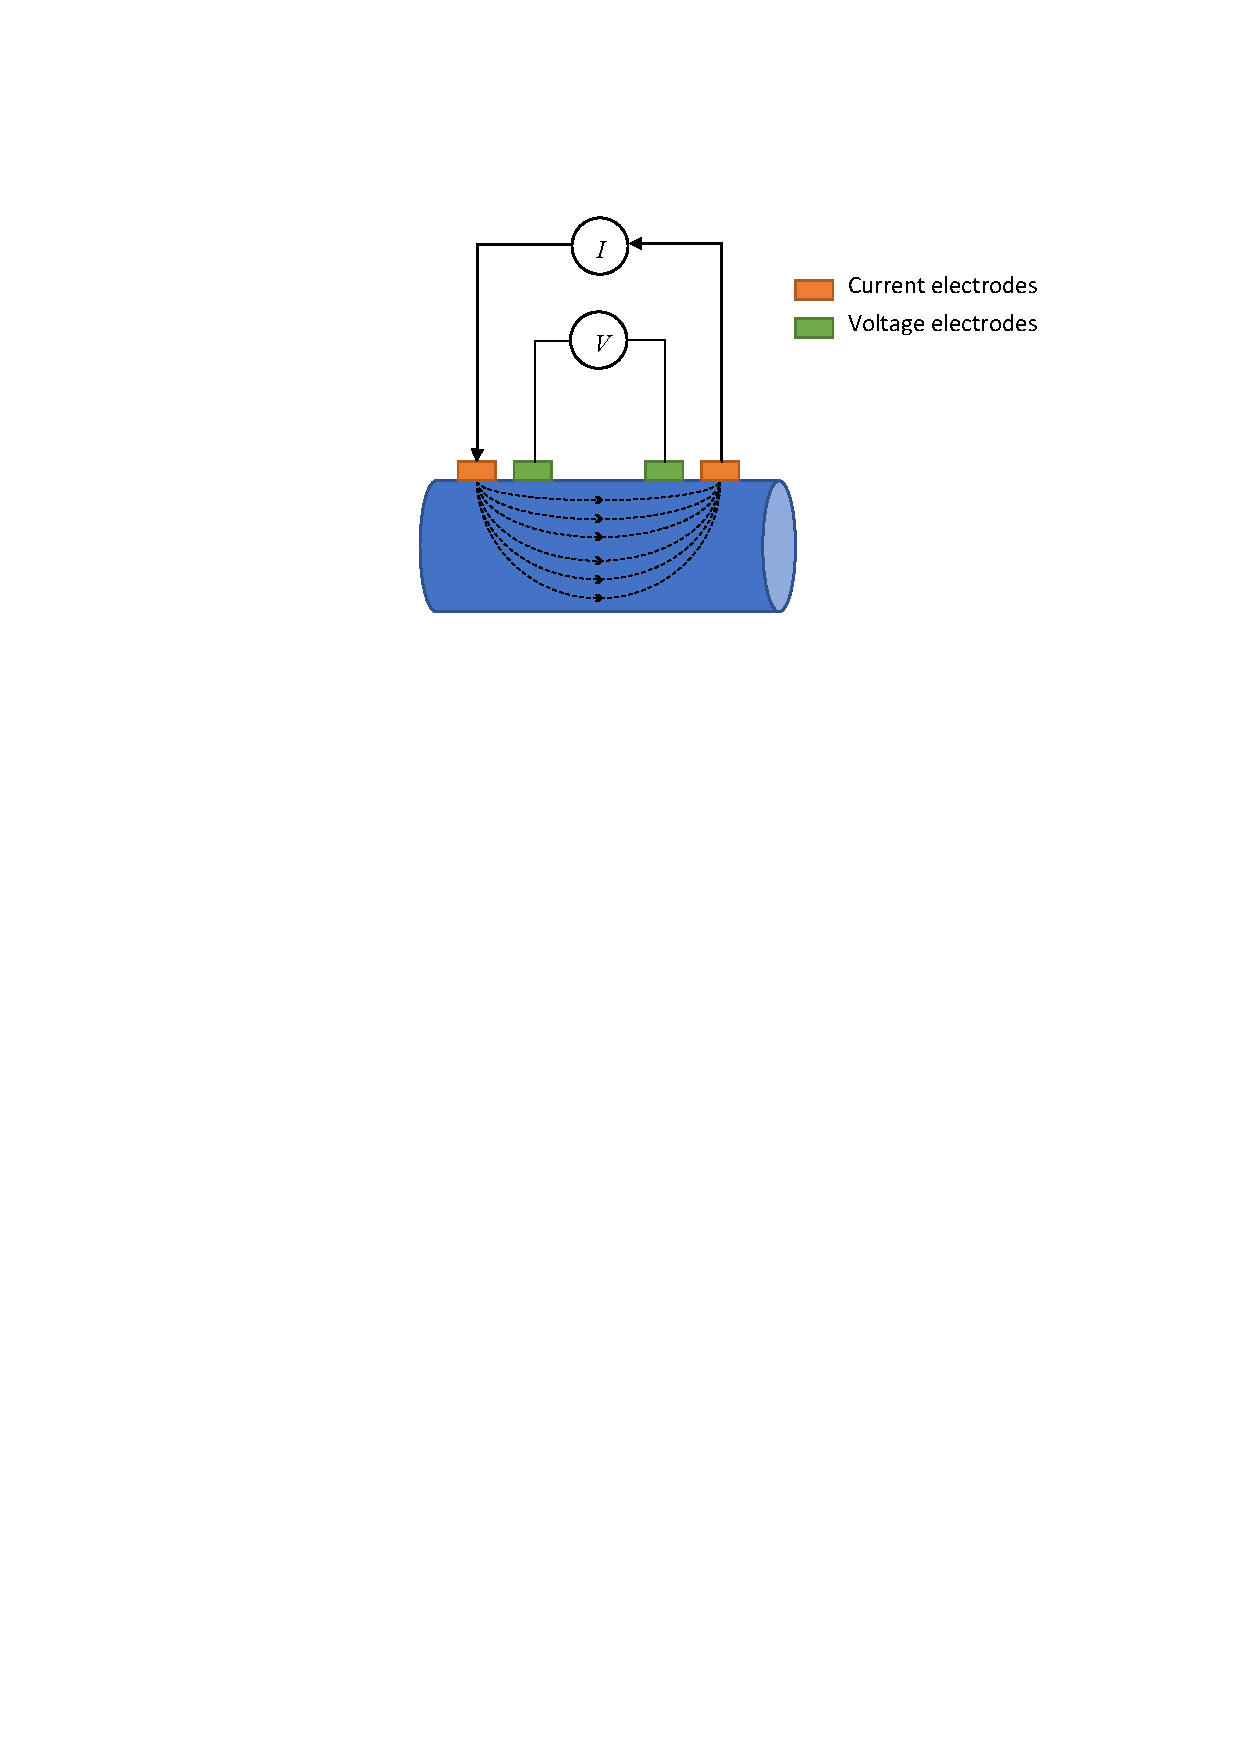
\includegraphics[width=0.5\textwidth,keepaspectratio]{tetrapolar_impedance}    
	\caption[Electrodes position in tetra-polar configuration]{Electrodes position in tetra-polar configuration. Outermost electrodes (current) inject current into the tissue. Inner electrodes sense the voltage drop caused by the tissue.}
	\label{fig:tetrapolar iPG}
\end{figure}

Another difference is the frequency used in iPG, to measure impedance plethysmography this varies according to the application but usually ranges from \SIrange{10}{100}{\kilo\hertz} \cite{songer2001tissue,casas1999vivo,kun1994tissue,ristic1997muscle}. This level of frequency is large enough to avoid any muscle stimulation that could be harmful to the patient. 

The electrical currents used by this method are in the range of few micro-amperes (\si{\micro\ampere}) to few milliamperes (\si{\milli\ampere}), keeping it within the limits of patient safety as described in section \ref{section impedance current in body}. Clearly, the higher the current, higher the voltage output response as per Ohm's law ($v = R \times i$) because the body segment behaves like a resistor. It must be noted that for patient safety, it is recommended to inject current instead of voltage. The reason for this is that circuits can limit the amount of injected electrical current and have a better control in the amplitude of the waveform. In the end, the amount of current required to obtain a clean signal depends on the geometry of the volume under test, the electrodes geometry and the physiological characteristics of the tissue. 

The data presented by an impedance device can be displayed as a real or imaginary part of the impedance. However, operating at this frequencies has been demonstrated that there is not much difference between the real part and the modulus of the measurement. In fact, the imaginary part of the signal is less than \SI{12}{\degree} \cite{jaffrin1979quantitative}. Therefore, the modulus of an impedance plethysmography measure provides enough information about the change of volume in a limb section \cite{anderson1984impedance}. Although, the phase might become important if higher frequencies are used to isolate particular tissue or physiological event.

\begin{figure}[!htpb]
	\centering
	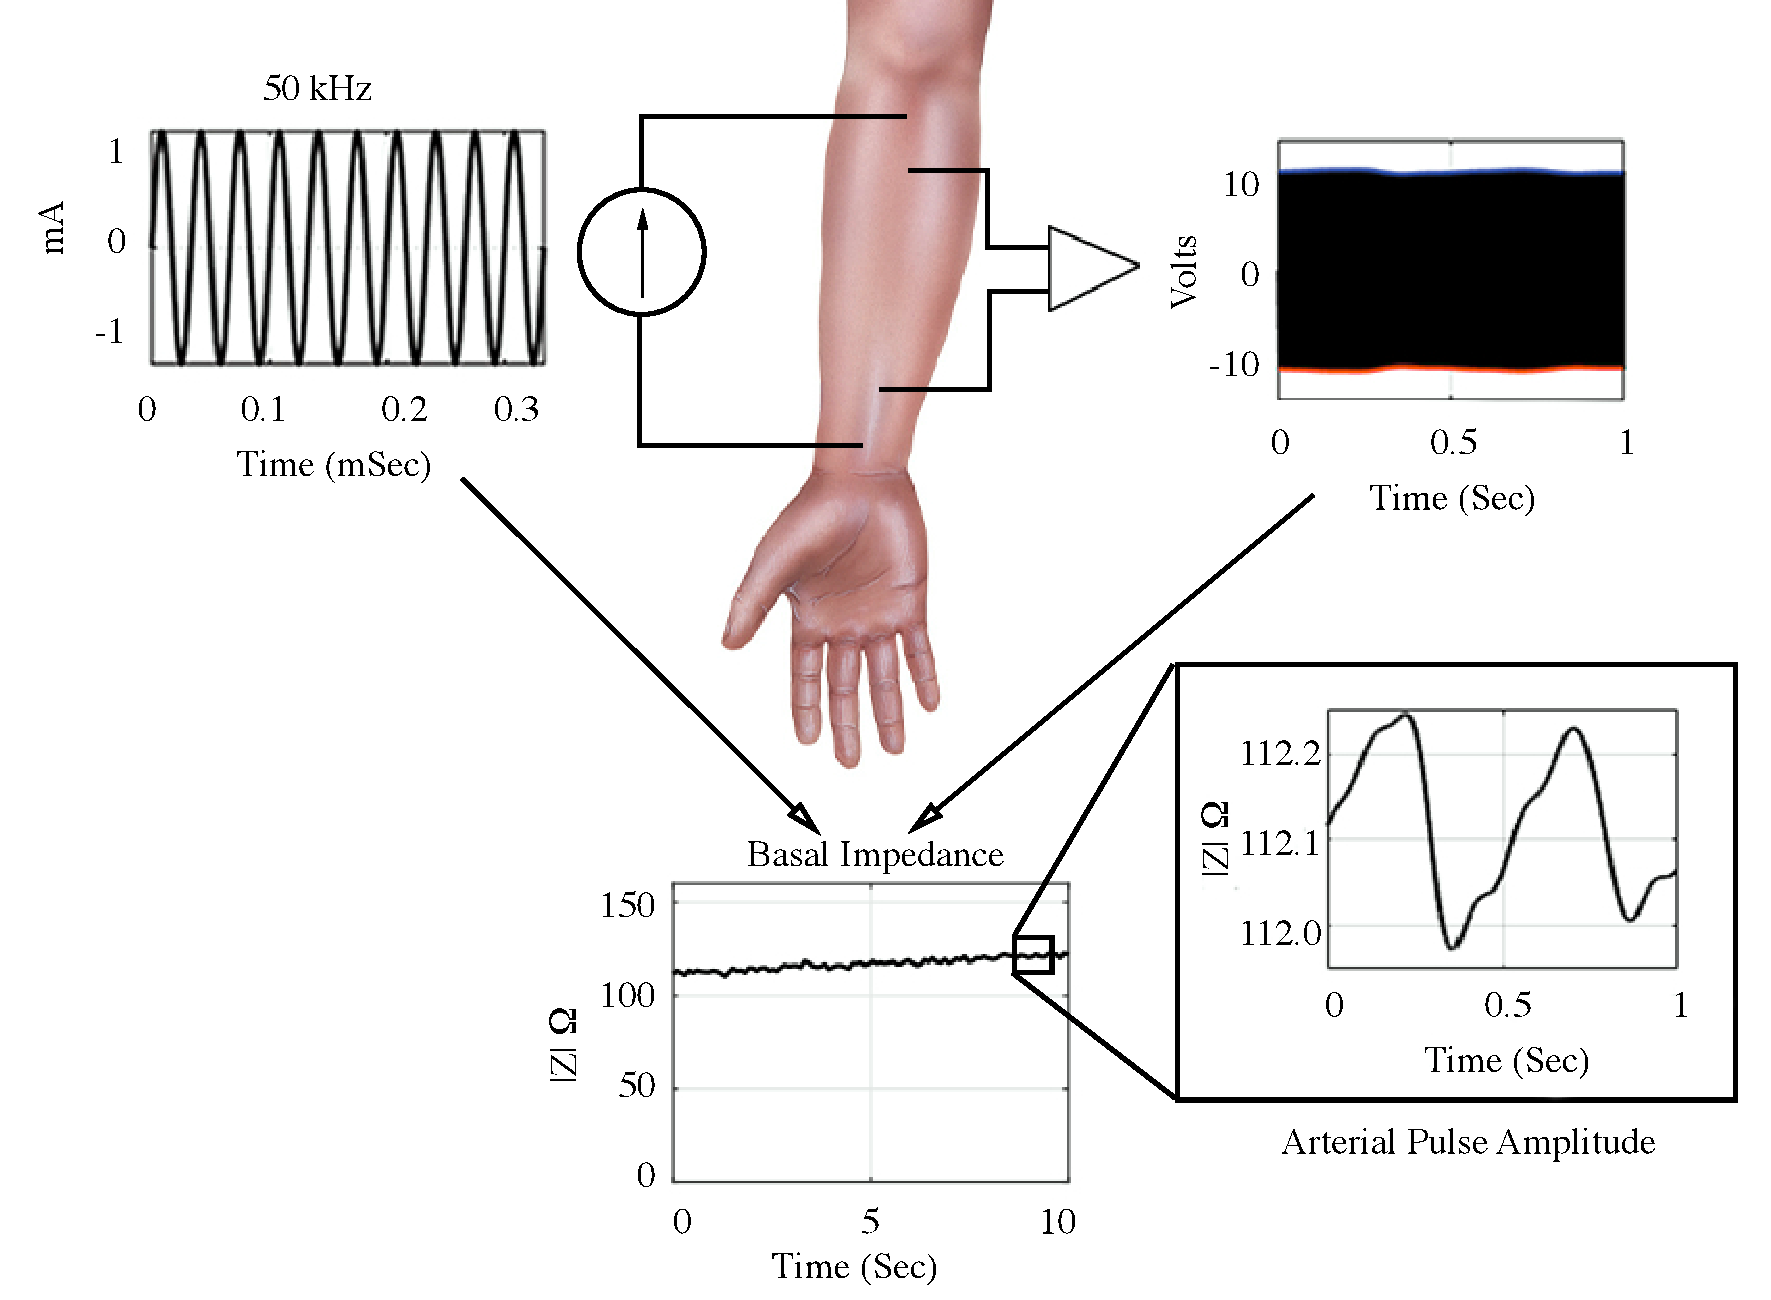
\includegraphics[width=\textwidth,keepaspectratio]{figure15}    
	\caption[How to get an impedance plethysmography waveform]{An impedance plethysmography waveform ban be obtained by applying a constant current. And sensing the resultant voltage. The division between the potential and the current provides the impedance module which is the basal impedance. Within the basal impedance the arterial pulse amplitude can be seen.}
	\label{fig:envelope iPG}
\end{figure}

In short, as the figure \ref{fig:envelope iPG} describes, obtaining an impedance plethysmography signal can be achieved by injecting the required current into the tissue at a specific frequency. One of the most common signals is \SI{50}{\kilo\hertz}. Once the electrical signals pass to the electrodes,  it is transformed into ionic conduction. The interaction of current with the tissue generates a drop of voltage that can be detected by the sensing electrodes. From the electrical point fo view, an amplitude modulated voltage waveform is generated from the tissue. However, this modulation which is synchronous to the heart cycle only represents \SI{0.1}{\percent} of the waveform \cite{anderson1984impedance}. 
The impedance modulus is obtained using Ohm's law (equation \ref{eq:|Z|}). The resultant impedance is known as either basal impedance (BI) or resting baseline impedance (RBI). Moreover, the dynamic signal within it is known as arterial pulse amplitude (APA). 
 
 \begin{align}
 	\label{eq:|Z|}
 	\left| Z \right| = \frac{v}{i}
 \end{align}


%********************************** %Second Section  *************************************
\subsection{Blood contribution to impedance} %Section - 3.2.1
As it has been described impedance plethysmography relies on the change of volume caused by blood vessels filling up all along the cardiac cycle. Nonetheless, blood is highly conductive and influences the amplitude of the waveform. However, there are also particular properties that might modify its intrinsic signal. In one of the earliest research about the conductivity of blood, Sigman et al.~\cite{sigman1937effect} demonstrated that resistivity of blood depends on its flow. It was found that when blood velocity decreased from \SIrange{10}{40}{\centi\meter\per\second} its resistivity fell roughly \SI{7}{\percent}. Furthermore, it was found that haematocrit and temperature are also factors that affects the blood resistivity \cite{yamakoshi1980noninvasive}. However, in an in-vivo setting the temperature remains nearly constant. Blood can be simplified as a suspension of particles (erythrocytes or RDC) with a high resistivity floating in a conductive medium (plasma). The rest of blood’s cells do not represent a great component in the change of impedance because of its small size in comparison with the erythrocytes (see table \ref{table:cell}). In fact, the Sigman effect is not presented in either plasma or electrolytes~\cite{tremper1990principles}.  

It has also been proved that blood is electrically anisotropic because of the orientation of the RBC’s \cite{Visser1992Electric}. Moreover, geometry and orientation also affect the reading of resistivity. Which also means that direction of measurement also affects the readings. 

\subsection{Impedance plethysmography waveforms}
\label{section iPG waveforms}
The impedance plethysmography provides information about the venous and arterial circulatory properties within a segment of the body. The impedance waveform is composed of a constant impedance value (basal impedance) and a dynamic component within it (arterial pulse amplitude). However, it is possible to obtain details about peripheral venous circulation when occluding a limb proximally. This kind of method is known as venous occlusion plethysmography (VOP).

\begin{figure}[!htpb]
	\centering
	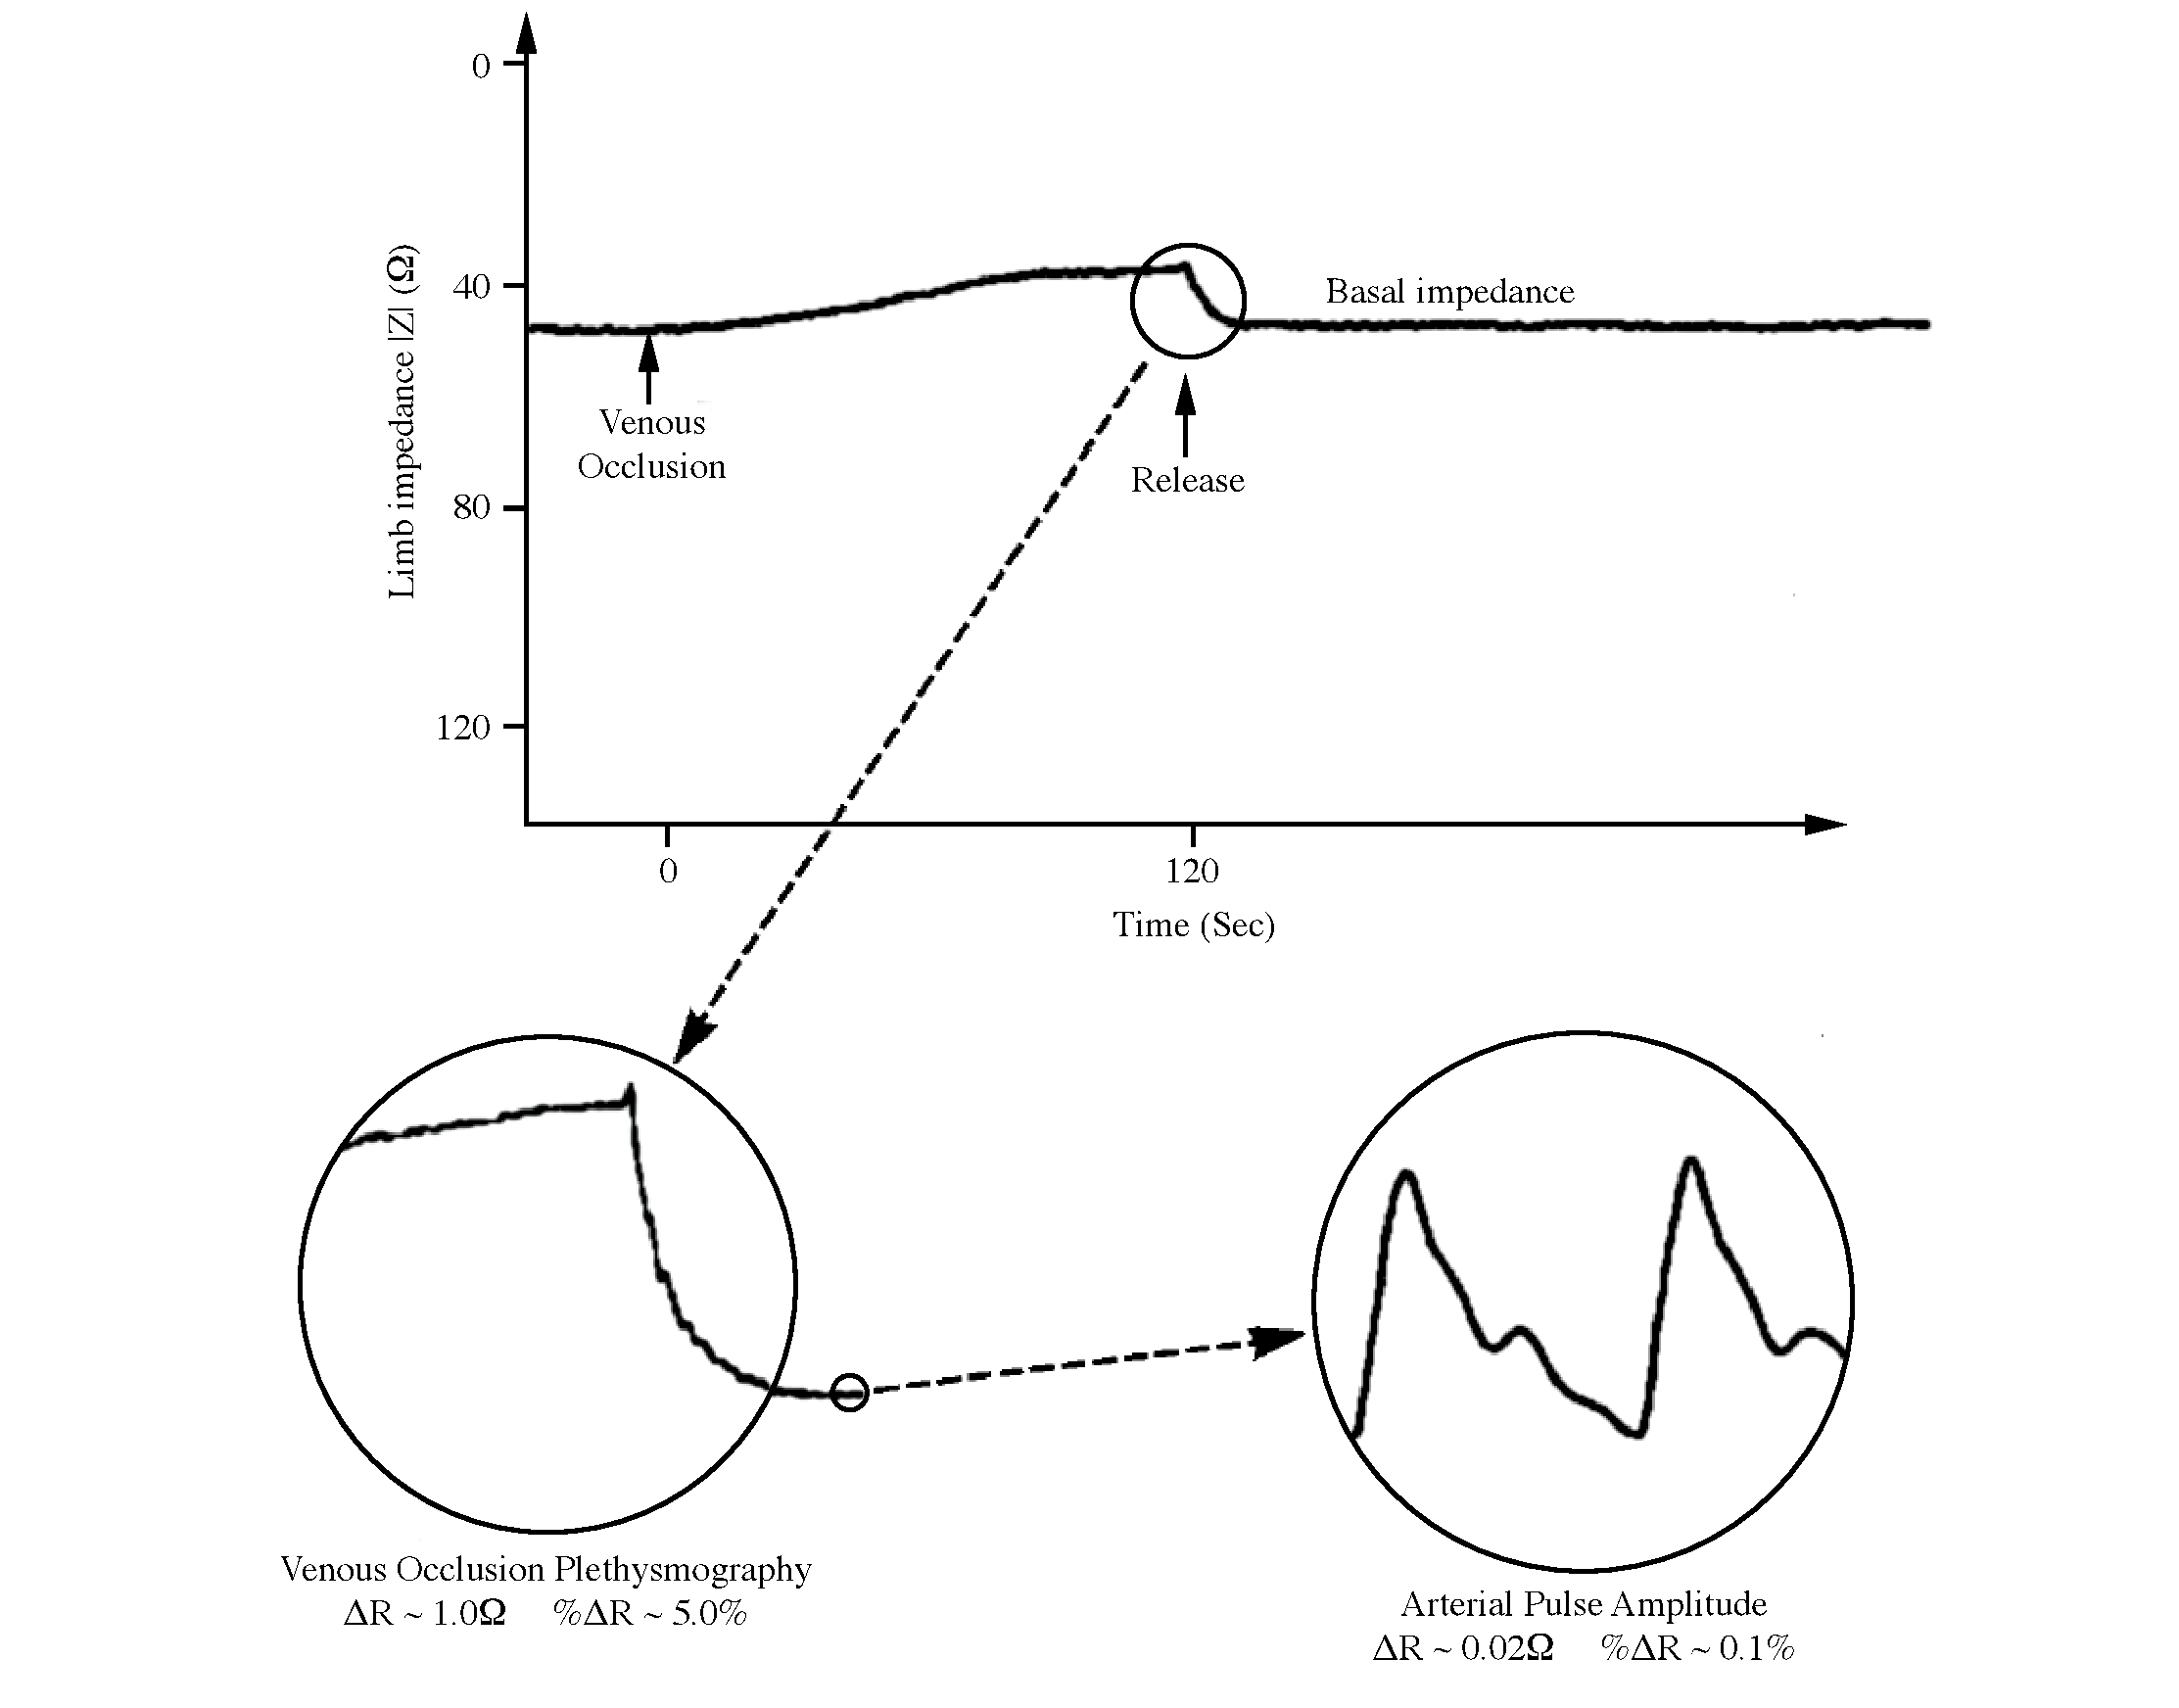
\includegraphics[width=\textwidth,keepaspectratio]{figure16}    
	\caption[Signal from an impedance plethysmography device]{An impedance plethysmography device can produce three signals. 1) the basal impedance or resting baseline resistance 2) by using a blocking venous return at (\SIrange{40}{50}{\mmHg}) is possible to extract the venous occlusion plethysmography wave 3) within the basal impedance is located the arterial pulse amplitude that changes with the heart beat. Adapted from \cite{anderson1984impedance}}
	\label{fig:iPG signals}
\end{figure}

Figure \ref{fig:iPG signals} shows the three different components of an impedance plethysmography waveform. The signal consists of the following components: basal impedance or resting baseline impedance (RBI), venous volumes changes and arterial pulses. 

\subsubsection{Basal impedance}
Also knows as the resistive baseline impedance, this is the most significant data obtain from an impedance plethysmography device (see figure \ref{fig:iPG signals}). The main contributors to this impedance are muscles, blood and bones. The resistivity of muscles is about \SIrange{200}{300}{\ohm\cm}, while the resistivity of bone and fat is greater than \SI{2000}{\ohm\cm} and the blood resistivity is about \SI{150}{\ohm\cm} \cite{gabriel1996dielectric}. Therefore, this combination of impedances can be expressed as a parallel model of resistances where muscle and blood which are the main contributors of the RBI. The range of this impedance value is from \SIrange{10}{100}{\ohm}. 

It has been demonstrated that is possible to gather information about the development of ischemic tissue by studying the changes of baseline during a time. Some studies have shown that there is an increase in the impedance value during ischemic events in the bandwidth of \SIrange{1}{100}{\kilo\hertz} in different kind of tissue \cite{songer2001tissue,casas1999vivo,kun1994tissue,ristic1997muscle} which is within the frequency measurement of iPG. 

\subsubsection{Venous occlusion plethysmography}
The second signal that obtained from the baseline signal provides information about the venous volume changes. Variations in the venous volume tone occur naturally during respiration which causes a modulation of the signal during the respiratory cycle between \SIrange{0.2}{0.3}{\hertz}. However, by occluding the venous return is possible to produce larger volume variations which are represented as a greater displacement of the basal impedance of about \SI{1}{\Omega} or \SI{5}{\percent} from the mean value. 

The most common method to evaluate venous volume is known as venous occlusion plethysmography, which is quite common in the assessment of peripheral vascular diseases such as deep venous thrombosis. Impedance plethysmography VOP (see figure \ref{fig:iPG signals}) provides a similar result as other well-established methods such as strain gauge\cite{schraibman1975comparison} and air/water displacement techniques \cite{fleming1986comparison}. This method requires occluding the proximal section of the limb using a cuff with a pressure above the venous pressure usually about \SI{40}{\mmHg}.  The holding of the blood return increases the volume of the limb with each heart cycle. The accumulation of blood in the measured segment increases its conductivity reducing the total resistivity.  A deviation from up to \SI{10}{\percent} from the basal impedance can be achieved depending on the occlusive pressure, arterial inflow, venous tone, central venous pressure (CVP), and the capacity of the venous vascular bed. 

\subsubsection{Arterial pulse amplitude}
The third signal component of an impedance plethysmography is the arterial pulsations which are waveforms synchronous with the heart cycle (\SIrange{1}{2}{\hertz}). This signal is just a fraction of the total impedance; it is just \SI{0.1}{\percent} of the total impedance signal, approximately \SI{0.02}{\ohm} in the limbs of healthy young adults. Obtaining this signal can be quite challenging as its value lies close to noise levels. Therefore, the signal should be isolated by using sharp filters and averaging some pulses. Changes of the waveform shape are due to different reasons such as tissue volume, arterial inflow, arterial vessel compliance, proximal occlusion, peripheral resistance as well as electrodes topology, geometry and location.  Changes in the signal amplitude is an indicator of arterial problems. For instance, with age arteriosclerosis reduces the arteries elasticity. Hence the arterial pulse amplitude reduces in magnitude.

\section{Conclusion}
Electrical impedance is the response that any conductive medium presents to an alternating current or voltage. It is frequency dependent and can be described as resistive ($R$) or reactive ($X$), which is determined by the resultant signal being in phase with the source or not. When applied to the human body it can be referred as bioelectrical impedance, which is a non-invasive method that allows analysing changes in the human body, using harmless and imperceptible AC. The current applied to any part of the body should be within the limits of patient safety, according to the literature any current below \SI{5}{\mA} is a good option but is also frequency dependent. 

Electrical impedance applied to humans can examine the health of tissue as well as changes in blood volume. The measurements produced by this method are due to the ions transport in tissue when a set of electrodes converts electrical current into ionic conduction. Bioelectrical impedance measurements can perform whole body measurements as well as local body segments. It can be applied using either single or multiple frequencies, or also perform analysis over a wide range of the spectrum. 

Bioelectrical impedance plethysmography measures the change of blood in segments of the human body. It is commonly used in a tetra-polar configuration where a pair of electrodes inject current and a second couple measures the voltage drop. Instruments utilising this technology produce two type of data by itself, one known as \textit{basal impedance} is the whole impedance contribution of bones, muscle, fatty tissue, skin and blood. In normal conditions, this signal tends to be unchangeable in time. However, within it lies another small signal that contains information of the arterial pulsations, known as \textit{arterial pulse amplitude}.

%********************************** %Nomenclatures in chapter  **************************************
\nomenclature[z-EM]{EM}{Electromagnetic}
\nomenclature[z-EIS]{EIS}{Electrical impedance spectroscopy}
\nomenclature[z-BLM]{BLM}{Bilayer lipid membrane}
\nomenclature[z-DLC]{DLC}{Dual layer capacitance}
\nomenclature[z-GSR]{GSR}{Galvanic impedance response}
\nomenclature[z-EWC]{EWC}{Extracellular water content}
\nomenclature[z-IWC]{IWC}{Intracellular water content}
\nomenclature[z-ICG]{ICG}{Impedance cardiography}
\nomenclature[z-PVT]{PVT}{Proximal vein thrombosis}
\nomenclature[z-BMI]{BMI}{Body mass index}
\nomenclature[z-BIVA]{BIVA}{Bioelectrical impedance vector analysis}
\nomenclature[z-SVR]{SVR}{Systemic vascular resistance}
\nomenclature[z-DSP]{DSP}{Digital signal processors}
\nomenclature[z-FFM]{FFM}{Free-fat mass}
\nomenclature[z-TBW]{TBW}{Total body water}
\nomenclature[z-ALS]{ALS}{Amyotrophic lateral sclerosis}
\nomenclature[z-BCM]{BCM}{Body cell mass}
\nomenclature[z-IEC]{IEC}{International Electrotechnical Commission}
\nomenclature[z-VF]{VF}{Ventricular fibrillation}
\nomenclature[z-RF]{RF}{Radio frequency}
\nomenclature[z-RMS]{RMS}{Root mean square}
\nomenclature[z-BI]{BI}{Basal impedance}
\nomenclature[z-RBI]{RBI}{Resting baseline impedance}
\nomenclature[z-APA]{APA}{Arterial pulse amplitude}
\nomenclature[z-VOP]{VOP}{Venous occlusion plethysmography}
\nomenclature[z-CVP]{CVP}{Central venous pressure}
\nomenclature[z-GSR]{GSR}{Galvanic impedance response}
\nomenclature[z-BIA]{BIA}{Bioelectrical impedance analysis}